%%% CLASS SETTING %%%
\documentclass[letterpaper, 12pt]{article}
\usepackage{natbib}
\usepackage[margin=1in]{geometry} % sets page layout 
\bibpunct[, ]{(}{)}{,}{a}{}{,} % sets the punctuation of the bibliography entires.
\usepackage{authblk} 

%%% Paper Information %%%
\title{Local Bandwagoning and National Balancing: How Uninformed Voters Respond to the Partisan Environment} % set the title of the document
\author{Gento Kato\thanks{Gento Kato is Ph.D. Student, Department of Political Science, One Shields Avenue Davis, CA 95616 (gkato@ucdavis.edu). The previous version of this paper was presented at the 77th Annual Midwest Political Science Association Conference, Palmer House Hilton, Chicago, IL, April 6, 2019. The latest version of this paper is available at \texttt{https://github.com/gentok/UninformedChoice}.}}
\affil{University of California, Davis}
\date{Last Update: September 9, 2019}

% Other Packages/Settings
\usepackage{amsfonts, amsmath, amssymb, bm} %Math fonts and symbols
\usepackage[format=hang, justification=centering]{caption}
\usepackage{dcolumn, multirow} % decimal-aligned columns, multi-row cells
\usepackage{booktabs} % Table formatting
\usepackage{graphicx, subfigure, float} % graphics commands
\usepackage[colorlinks=true, citecolor=blue]{hyperref}
\usepackage{setspace}% allows toggling of double/single-spacing
\doublespace % set document spacing to double
%\usepackage{endnotes}
%\let\footnote=\endnote
% Draw figure
% \usepackage{tikz}
% \usetikzlibrary{calc}
% Add note to Figures
\newcommand{\floatnote}[1]{\vspace{\abovecaptionskip}\caption*{\textbf{Note:} #1}\vspace{-\abovecaptionskip}}
% Change section font
\usepackage{sectsty} 
\sectionfont{\fontsize{14}{14}\selectfont} 
\subsectionfont{\fontsize{12}{12}\selectfont\itshape} 
\subsubsectionfont{\fontsize{12}{12}\selectfont} 
% Move figures to the last
%\usepackage[figuresonly]{endfloat} %nomarkers, to avoid markers
%\renewcommand{\listoffigures}{} % but suppress these lists

\begin{document}

\begin{titlepage}
    
    \singlespace
    \maketitle
    \thispagestyle{empty}
    
    % \clearpage
    % \thispagestyle{empty}
    
    \begin{abstract}
        Scholarly debate on civic competence often assumes that political knowledge is the prerequisite for systematic and ``correct'' decision-making. Uninformed voters, then, are portrayed as unsystematic and misguided decision-makers. The current study challenges this assumption by arguing that uninformed voters may not rely on (potentially misguided) individual preferences but rather refer to the partisan environment, the partisan voting patterns in past elections, to guide their decisions. The analysis of Cooperative Congressional Election Study (CCES) and American National Election Studies (ANES) provides the supporting evidence to this claim. Uninformed voters respond to the partisan environment in two ways: First, they \textit{bandwagon} with the local partisan environment; second, they \textit{balance} against the national partisan environment. The results provide the view of uninformed voters as more systematic and effective decision-makers than previously suggested.
    \end{abstract}
    \end{titlepage}
    
    \clearpage
    \doublespace

    \par In the studies of voter competence, the non-randomness and ``correctness'' of voting decisions are believed to be strictly increasing in the level of political knowledge. Uninformed voters, under this view, are portrayed as the most unsystematic and misguided decision-makers. Their individual preferences are unstable \citep{Converse1964thna, Zaller1992thna}, internally inconsistent \citep{Broockman2016apto}, or misinformed \citep{Kuklinski2000mian, Fowler2014thpo}. The evidence often leads to the conclusion that uninformed voting cannot be explained systematically. Any deviation of uninformed votes from informed votes \citep{Bartels1996unvo} is attributed to biased preference formation of uninformed voters. Yet, this conclusion is the assumption rather than the explanation of the nature of uninformed voting. Previous studies rarely explore the possible reasoning behind uninformed voting patterns.
    
    \par Given this gap in literature, this paper asks the following research question: \textit{how can the behavior of uninformed voters be systematically explained?} There are two propositions. First, I argue that individual preferences \textit{do not} explain the behavior of uninformed voters. Uninformed voters know that their preferences are weakly reasoned and potentially biased, and thus have no incentive to use their own preference to inform their decisions. Second, partisan environment, represented by aggregated partisan voting patterns from past elections \citep{Miller1956onpo, Putnam1966poat}, explains uninformed voting. If a voter is informed, he or she has no reason to refer to partisan contexts. For uninformed voters, however, two contrasting sets of logic, \textit{bandwagon} and \textit{balance}, explain how and why contexts can be useful for their voting decisions.
    
    \par This paper consists of two studies that assess the implication of context-based uninformed voting. Both studies test propositions through the analysis of American presidential elections. The first study assesses the role of local partisan environments through the 2008 and 2016 Cooperative Congressional Election Study (CCES), and the second study examines the role of national partisan environments through 1972--2016 American National Election Studies (ANES). 
    
    \par The empirical results show that uninformed and informed voters base their decisions on separate sets of resources. Partisan environments explain uninformed voting but not informed voting; individual perceptions of ideological proximity and valence differential explain informed voting but not uninformed voting. Furthermore, the role of partisan context changes by the level of context: uninformed voters bandwagon with local partisan environments but balance against national partisan environments. 
    % The simulation results imply that especially when the knowledge level is highly unequal across partisan groups, the conditional strategy of context-based uninformed voting produces more favorable democratic outcomes than alternative strategies.
    
    \par The inquiry in the current paper sheds new lights on the studies of voting behavior. First, it helps to understand the decision-making process of uninformed voters. Previous empirical studies often emphasize the inconsistent and misguided nature of uninformed preferences, but this paper offers the picture of uninformed voters who can (at least partially) cope with this disadvantage. Second, it opens up a new way to assess voter competence. Instead of asking if voters are informed enough to acquire ``correct'' preference, we can ask whether the behavioral rules of uninformed voters contribute to the individual or social welfare. Having uncertain and ``incorrect'' individual preferences does not necessarily undermine the quality of democratic decision-making.
    
    \section*{Information Effects Unexplained}
    
    \par The capacity of citizens to make competent decisions is one of the main targets of endeavor in the studies of democratic voting behavior. Scholars repeatedly suggest that ordinary voters rarely hold a sufficient level of political knowledge to form consistent political preferences. American voters are uninformed about the wide range of political facts \citep{Dellicarpini1996wham}, and those ill-informed voters cannot hold a political ideology that is consistent across time and issues \citep{Converse1964thna, Zaller1992thna, Broockman2016apto}. While some argue that voters need only necessary signals, not the full set of factual knowledge, to form ``informed'' preferences \citep[e.g.,][]{Lupia1994shve}, it is shown that signaled preferences can be biased and misleading \citep{Kuklinski2000mian, Fowler2014thpo, Boudreau2015loin}.

    \par In the search for implications of this widely documented ignorance, scholars have been making the empirical assessment of ``information effects.'' They are interested in how uninformed voting patterns deviate from informed counterparts. In his canonical study, \cite{Bartels1996unvo} analyzes the presidential vote choice in the American National Election Study and demonstrates that informed and uninformed voters have different tendencies in how demographic characteristics influence the voting decisions. He further shows that those differential voting patterns have a sizable influence on aggregated electoral outcomes. Similarly, \cite{Arnold2012thel} analyzes Comparative Study of Electoral Systems (CSES) and shows that hypothetical fully informed voting may change the electoral outcome across a wide range of democracies. 
    
    \par The substantive implications of these empirical findings, however, are not always clear and generalizable. The interpretations of differences are mostly descriptive and rarely offer a systematic explanation. As a result, we have little understanding as to why there are differences between uninformed and informed voting and how they influence the democratic outcome. The next section introduces theories of voting that can offer those missing explanations. %to move the scholarly discussion forward.
    
    \section*{Uninformed Voting and the Partisan Environment}

    \par The accumulation of voting research offers several candidate explanations regarding how and why uninformed voting patterns differ from informed voting patterns. The most straightforward explanation is that uninformed voters make decisions based on the perception of the state of the world that deviates from the informed perception. This explanation implies that individual preferences (i.e., ideology and valence evaluation) predict uninformed and informed voting in the same manner; differences appear because less informed voters receive preference signals that are potentially more biased and less stable.

    \par Suppose that two candidates from two parties, $B$ and $R$, are running in a plurality election. The following probabilistic voting function can describe the above voting calculus:
    \begin{align}
        Pr(\text{Vote R})_i  &=  \Lambda\left( b_1\left( \left(\widehat{\delta_i-\Delta_{R}}\right)^2 - \left(\widehat{\delta_i-\Delta_{B}}\right)^2 \right) + b_2\left(\widehat{\Theta_{R} - \Theta_{B}}\right) + \gamma_i + \epsilon_i \right) \label{eq1} \\
        \widehat{\delta_i-\Delta_{R}} &= \delta_i-\Delta_{R} + \eta_{\Delta_R}(k_i) \label{eq2} \\
        \widehat{\delta_i-\Delta_{B}} &= \delta_i-\Delta_{B} + \eta_{\Delta_B}(k_i) \label{eq3} \\
        \widehat{\Theta_{R} - \Theta_{B}} &= \Theta_{R} - \Theta_{B} + \eta_{\Theta}(k_i) \label{eq4}
    \end{align}
    \noindent In \autoref{eq1}, the probability of voter $i$ choosing party $R$ is the inverse logit function $\Lambda$ of following components: The perception of relative proximity of $i$'s ideology $\delta_i$ to party $R$'s ideology $\Delta_R$ than to party $B$'s ideology $\Delta_B$ \citep{Downs1957anec}; the perception of valence or quality advantage (or disadvantage) of party $R$ over party $B$ candidates $\Theta_{R} - \Theta_{B}$ \citep{Adams2011whca}; utility from group identity $\gamma_i$ such as partisanship and demographic groups \citep{Campbell1964tham,Tajfel1986thso}; and other random disturbances $\epsilon_i$. $b_1, b_2 \geq 0$ are coefficients attached to relative ideological proximity and valance differential. \autoref{eq2}, \autoref{eq3}, and \autoref{eq4} show that the perception of ideological proximity and valence evaluation consists of true proximity or evaluation and error $\eta(k_i)$ (unobservable to $i$) drawn from some distribution $f_\eta(k_i)$. Both expected value (i.e., bias) and variance (i.e., instability) of $f_\eta(k_i)$ are shrinking in political knowledge $k_i \in [0,1]$ and converge to $0$ when $k_i=1$. In this model, uninformed voters (i.e., low $k_i$) make different choice than informed voters (i.e., high $k_i$) only because random errors are contaminating their perception of ideology and valence.

    \par However, there are reasons to expect that uninformed voters rely less on their perception of ideology and valence than informed voters do. Extending the voting model suggested in \cite{Downs1957anec}, \cite{Matsusaka1995exvo} argues that uninformed voters are less certain than informed voters about their perception of electoral preferences. While his primary interest is in the turnout decisions, his theory implies that uninformed voters, compared to informed voters, may discount their preferences when making vote choice. Empirical evidence supports this claim. For example, \cite{Dellicarpini1996wham} find that the predictive power of ideology in voting is weaker among less-informed voters. Therefore, the first hypothesis is constructed as follows:

    \begin{verse}
        H1: The less-informed that voters are, the less strongly the perception of ideology and valence explains their voting decisions.
    \end{verse}

    \par If uninformed voters do not rely on their individual preferences, are their voting decisions inherently based on identity and random disturbances? The long history of research on social context influence on voting suggests that is not necessarily the case. Even when voters do not possess the sufficient information to form their own preference with certainty, they may still learn and utilize the distribution of others' partisan preferences in the society (called \textit{partisan environment}). Voters obtain this knowledge from past election results and preferences of others in the social network. The second hypothesis states that the differences between informed and uninformed voting originate from the use of this contextual information:

    \begin{verse}
        H2: The less-informed that voters are, the more strongly a partisan environment explains their voting decisions. 
    \end{verse}

    \noindent Voters may respond to a partisan environment in either of two different ways: \textit{bandwagoning} and \textit{balancing}. Both patterns have theoretical and empirical support to validate their underlying logic. The following subsections explain why uninformed voters, and only uninformed voters, have a reason to bandwagon with or balance against the partisan environment.

    \subsection*{Bandwagoning}

    \par Bandwagoning indicates the pattern of behavior to vote in line with the majority in a partisan environment. This pattern of context-based voting is supported by ample empirical evidence. Early inquiries of local context and voting suggest that voters living under a highly skewed partisan environment, captured by partisan voting patterns in past election results, have a strong tendency to vote in line with the majority party \citep{Miller1956onpo, Putnam1966poat}. The collection of social network studies also finds that majority preference in one's political discussion network predicts voting decisions \citep{Huckfeldt1987nein, Huckfeldt1995cipo, Huckfeldt2014nobi}. In addition, experimental studies confirm bandwagoning behavior both in lab \citep{Bischoff2013soin, Morton2015whmo, Tyran2016exev} and online survey \citep{Roy2015anex,vanderMeer2016ofth, Dahlgaard2017hoel}. In those experiments, participants are randomly assigned to receive the signal about the majority preference (or the candidate/party winning the election) or not. The results show that receivers of the contextual signal are more likely to act in line with the majority than those who do not receive the signal.

    \par There are numbers of theoretical rationales as to why bandwagoning should occur \citep{Hardmeier2008thef}. While psychological explanations emphasize the natural instinct or ``feels good'' aspect of joining on the winner's side, voters may have a logical incentive to use majority preference as a heuristic to find ``correct'' choices in elections \citep{Lupia1994shve, Lau2001adan}.\footnote{The separate set of theoretical studies focuses on the role of bandwagoning to maximize the impersonal utility \citep{Coate2004grru, Feddersen2006thca, Feddersen2006thof} but this theory does not speak to the difference between informed and uninformed voters.} It is reasonable to expect that the heuristic-based bandwagoning is weaker among informed than uninformed voters because those with abundant resources to support their own preferences tend to be resistant to the reception of additional signals \citep{Zaller1992thna}. Empirical evidence is consistent with this claim. For example, the mock election experiment conducted by \cite{Huckfeldt2014nobi} shows that voting decisions of participants who are able to receive more private information about their preference are affected less by the preference signals obtained through communication with other participants. Similarly, the survey experiment conducted by \cite{Roy2015anex} indicates that the depth of obtained candidate information moderates bandwagoning behavior. \cite{Roy2015anex} design a mock election in which respondents can search for information about candidates. After the search, the random subset of participants receives the result of the pre-election polling that contains the information regarding the leading candidate in the election. The experiment results show that the bandwagoning effect of pre-election polling treatment is weaker for those who searched more information about candidates (i.e., informed voters) than for those who searched less (i.e., uninformed voters). 
    
    \par The heuristic explanation of bandwagnoning implicitly assumes that uninformed voters share the common preference with other voters in the same environment. In turn, the ideological homogeneity of the society would strengthen the relationship between a partisan environment and bandwagoning behavior. Under the context of American presidential elections, the ideological preferences are highly heterogenous at the national level. On the other hand, the patterns of racial and partisan geographic sorting (\citealt{Charles2003thdy,TamCho2013vomi} but \citealt{Mummolo2017whpa}) suggest that local distributions of ideological preferences are more homogenous than the national distribution. Local partisan environments often have a weak connection to winning or losing in the national election, but can be an effective heuristic in inferring how others with similar ideology vote.

    \par In sum, the third hypothesis suggests that bandwagoning is primarily occurring in response to the local partisan environment among uninformed voters:

    \begin{verse}
        H3: The more skewed the local partisan environment, the more likely uninformed voters (and not informed voters) vote with the majority party in the local partisan environment. 
    \end{verse}

    \subsection*{Balancing}

    \par Under the context of the American presidential system, scholars frequently discuss balancing in terms of vote switching in mid-term elections \citep{Alesina1995papo}. More generally, scholars understand balancing as the strategy of ideologically moderate voters to prevent policy outcomes from skewing overly toward one direction. While balancing tends to require the cognitively demanding task of understanding complex electoral and policy-making institutions, empirical studies show that many voters do get involved in balancing behavior under various contexts \citep{Kedar2005whmo, Kedar2006hovo, Folke2012gumi}.  
    
    \par In the scope of the current research, balancing is the pattern of behavior to vote against the majority in the partisan environment. The voting model presented in \cite{Feddersen1996thsw} explains why uninformed voters, and not informed voters, have an incentive to conduct such balancing. Their model categorizes voters into partisans, informed independents, and uninformed independents and explains the behavior of each type of voters. Through the equilibrium analysis, they show that informed independents and partisans vote for their individual preference, but uninformed independents vote to ``maximize the probability that the informed independent agents determine the winner'' \citep[][p.414]{Feddersen1996thsw}. To achieve this purpose, when they vote, uninformed independents have an incentive to balance out the partisan imbalance in society. This balancing increases the likelihood of informed independents determining the outcome, which favors the interest of uninformed independents. 

    \par To get an intuitive sense of balancing, back to \autoref{eq1}. $B$ and $R$ partisans (i.e., having large difference between $\left(\widehat{\delta_i-\Delta_{R}}\right)^2$ and $\left(\widehat{\delta_i-\Delta_{B}}\right)^2$) have a strong ideological preference toward parties, so they almost always vote for their own party. Here, ideologically moderate voters benefit more from electing the \textit{better} party in terms of common quality (i.e., $\Theta_{R} - \Theta_{B}$ differential). Informed voters know, while uninformed voters don't know, which party has the better quality. The balancing logic suggests that moderate uninformed voters are less likely to vote for the parties with a larger number of partisans. This balancing behavior increases the likelihood of a moderate informed voter, whose decision should benefit moderate uninformed voters, being the median pivotal voter in the election. The series of lab experiments with university student subjects provide the empirical support for this mechanism \citep{Battaglini2008inag, Battaglini2010thsw}.
    
    \par The balancing concerns the type of voters determining the electoral outcome. In American presidential elections, the outcome of interest is at the national level.\footnote{Technically, American presidential election is a two-step process. The national-level vote share does not always determine, but plays an important role in the electoral outcome.} It makes sense for uninformed voters to balance their votes against the national than the local partisan environment. Therefore, the fourth and last hypothesis of this paper is constructed as follows:

    \begin{verse}
        H4: The more skewed the national partisan environment, the more likely uninformed voters (and not informed voters) vote against the majority party in the national partisan environment. 
    \end{verse}

    \subsection*{The Model of Context-based Uninformed Voting}

    \par If implications from H1, H2, H3, and H4 hold, \autoref{eq1} can be modified as follows: 
    \begin{align}
        Pr(\text{Vote R})_i  =&  \Lambda( k_i \times \left( b_1\left(\widehat{(\delta_i-\Delta_{R})}^2 - \widehat{(\delta_i-\Delta_{B})}^2 \right) + b_2\left(\widehat{\Theta_{R} - \Theta_{B}}\right) \right) \notag \\
        &+ (1-k_i) \times \left( b_3\pi_R(Local) - b_4\pi_R(National)\right) + \gamma_i + \epsilon_i ) \label{eq5} 
    \end{align}
    \noindent Modified part of \autoref{eq5} is expressed as the weighted average of preference perceptions and partisan environments. While the role of ideology and valence perceptions is strengthening in political knowledge $k_i$ (H1), the role of partisan environments is strengthening in the lack of knowledge $1-k_i$ (H2). In the second line, $\pi_R \in [0,1]$ represents party $R$ supporters' proportion in a given partisan environment and $b_3, b_4 \geq 0$ are coefficients attached to each partisan environment. Then, the probability of $R$ vote is increasing in the local partisan environment $\pi_R(Local)$ (H3) and decreasing the national partisan environment $\pi_R(National)$ (H4).

    \section*{Study 1: Local Partisan Environment and Uninformed Voting}

    \par This section examines the relationship between local partisan environment and vote choices in American presidential elections. Specifically, I use the Cooperative Congressional Election Study (CCES) conducted in 2008 and 2016. Each respondent is matched with past presidential election outcomes aggregated at the level of their local environment (i.e., state and county of residence). The election data are obtained from CQ Press Voting and Election Collections.\footnote{\url{http://library.cqpress.com/elections}. Accessed through subscription at the library of the University of California, Davis.}
    
    \par The advantage of using CCES for the analysis of the local partisan environment is that the dataset includes a large number of respondents from different locations across the United States, providing sufficient variations and data points at both county and state level. While CCES recruits respondents from online and thus the sample is not nationally representative, it is validated that most of the actual election results do fall within the 95\% confidence interval of the weighted estimates from CCES samples \citep{Ansolabehere2011guto, Ansolabehere2017guto}. The following analysis applies weights provided by CCES organizers to correct for the potential bias in sampling.\footnote{Since the analysis includes the post-election variable of vote choice, post-election weights are used for CCES2016. General weights are used in CCES2008 because post-election weights are not provided.}

    \subsection*{Variables}
    
    \par The primary dependent variable for this study is the vote choice in presidential elections. To simplify the analysis, I focus on the binary choice between Republican and Democratic candidates and thus drop reported third-candidate choosers and abstainers from the analysis.\footnote{Turnout decision and third-candidate voting deserves a separate set of discussions, but that is not the central focus of this paper.} To explain the dichotomous vote choice, four sets of predictors are relevant. First, the measure of \textit{political knowledge} is constructed from eight factual test questions in CCES concerning the knowledge of the majority party in legislatures and party name of incumbent politicians. The correct answers are aggregated to construct the information scale (the Cronbach's alpha is 0.84 in 2008, 0.87 in 2016). The final score is normalized between 0 and 1.
    
    \par Second, the measures of \textit{local partisan environment} are constructed by linking the results of past elections with each respondent in CCES. Past electoral outcomes may not be the direct representation of the partisan composition of the society, but the evident pattern in the past elections gives a strong clue as to how partisan preferences are distributed within society. From CQ Press Voting and Election Collections, I collected county and state level outcomes of presidential elections. Using two-party Republican vote share in each local unit, the adapted versions of \textit{Cook Political Report} Partisan Voter Index (PVI)\footnote{\url{https://www.cookpolitical.com/pvi}} are calculated. State level PVI uses the following formula for each state $i$ and election cycle $t$: 
    \begin{align*}
    \textit{(State PVI)}_{t,i} = \{ & (\textit{(State Republican Share)}_{t-1, i} - \textit{(National Republican Share)}_{t-1}) + \\  
    &(\textit{(State Republican Share)}_{t-2, i} - \textit{(National Republican Share)}_{t-2}) \}/2
    \end{align*}    
    \noindent In the above formula, $t$ represents the current election, and $t-1$ and $t-2$ represent the previous two elections. $\textit{(State Republican Share)}_i$ indicates two-party vote share of the Republican party against the Democratic party in state $i$. Thus, \textit{State PVI} represents the average advantage of Republican party vote share over the Democratic party, relative to the national tendency in the previous two elections. Two elections are averaged to determine the long-term trend in a partisan environment. The positive scores indicate the advantage in Republican vote share in percentage points, and the negative scores indicate the advantage in Democratic vote share in percentage points. In addition, county level PVI measures are calculated using the following formula:
    \begin{align*}
        \textit{(County}& \textit{PVI)}_{t,i,j} = \\
        \{ &(\textit{(County Republican Share)}_{t-1, j} - \textit{(State Republican Share)}_{t-1,i}) + \\  
        &(\textit{(County Republican Share)}_{t-2, j} - \textit{(State Republican Share)}_{t-2, i}) \}/2
    \end{align*}    
    \noindent Notice that the above formula adjusts the PVI for county $j$, not by national-level vote shares but by state-level vote shares. Therefore, the measure captures the partisan deviation of each county from the state average. Consequently, the correlations between state and county or district PVI are very low (ranges from $-0.01$ to $0.14$) and inlusion of both variables in one model makes sense.
    % (-0.086 for 08 county,  -0.01108314 for 08 district  -0.04256889 for 16 county -0.1421199 for 16 district)
        
    \par The third set of predictors is \textit{individual preferences}. relative ideological proximity (based on squared ideological distance from each candidate, ranges from $-36$ to $36$), and the retrospective economic evaluation (ranges from $-2$ to $2$). All variables are scaled so that the higher score indicates preference toward Republican party candidates (see Online Appendix A for detailed constructs). All preference variables are based on the subjective perceptions. In contrast to objective measures that aim to capture ``true'' preference of voters, the subjective preference, even when it is potentially biased, is most likely to influence voting decisions. 

    \par The last sets of predictors are \textit{partisanship} and \textit{demography}, including party identification (ranges from $-3$ to $3$), gender, age, race, income, education, and religiosity. The theory has no specific expectations regarding how the impact of partisanship demographic variables interact with political knowledge, but those variables are included in the analysis to control for the baseline tendency in voting behavior. 
    
    \subsection*{Model}

    \par The predictive model intends to identify the differential behavioral patterns between uninformed and informed voters. This paper follows the approach taken by \cite{Bartels1996unvo} to include the complete set of linear interactions between predictors and political knowledge. 
    %The final model appears as follows:
    % \begin{align*}
    % Pr&(\text{Vote Republican})_i = \Lambda\{\\
    % &\alpha + \beta (\text{Political Knowledge})_i +  \\
    % &\delta_{1-2} (\text{Local Partisan Environments})_i + \gamma_{1-2} (\text{Local Partisan Environments})_i \times \text{Knowledge}_i + \\
    % &\delta_{3-5} (\text{Individual Preferences})_i + \gamma_{3-5} (\text{Individual Preferences})_i \times \text{Knowledge}_i + \\
    % &\delta_{6-10} (\text{Demographics})_i + \gamma_{6-10} (\text{Demographics})_i \times \text{Knowledge}_i \}
    % \end{align*} 
    % \noindent 
    Assuming that a linear relationship exists between political knowledge and the impact of each predictor, this method allows estimation of conditional coefficients of each predictor at different levels of political knowledge. After the estimation, I generate the conditional coefficient of each predictor for fully informed (political knowledge $= 1$) and uninformed (political knowledge $=0$) voters.

    \par I use logistic regression to estimate the impact of predictors on vote choice (Democrat = 0, Republican = 1). Standard errors are clustered by states and counties to incorporate common behavioral tendencies within those areas.\footnote{The results are robust to the alternative specification using mixed effects logistic regression with states and counties random effects. See Online Appendix.} In addition, the multiple imputation procedure \citep{King2001anin} is used to handle the missing responses in the dataset. The presented results are the average from analyses of five imputated datasets.
    
    \subsection*{Results}
    
    \begin{figure}[t!]
        \caption{The impact of local partisan environments and individual preferences on informed and uninformed presidential vote choice in CCES (2008, 2016)}
        \label{fig:ccescoefplot}
        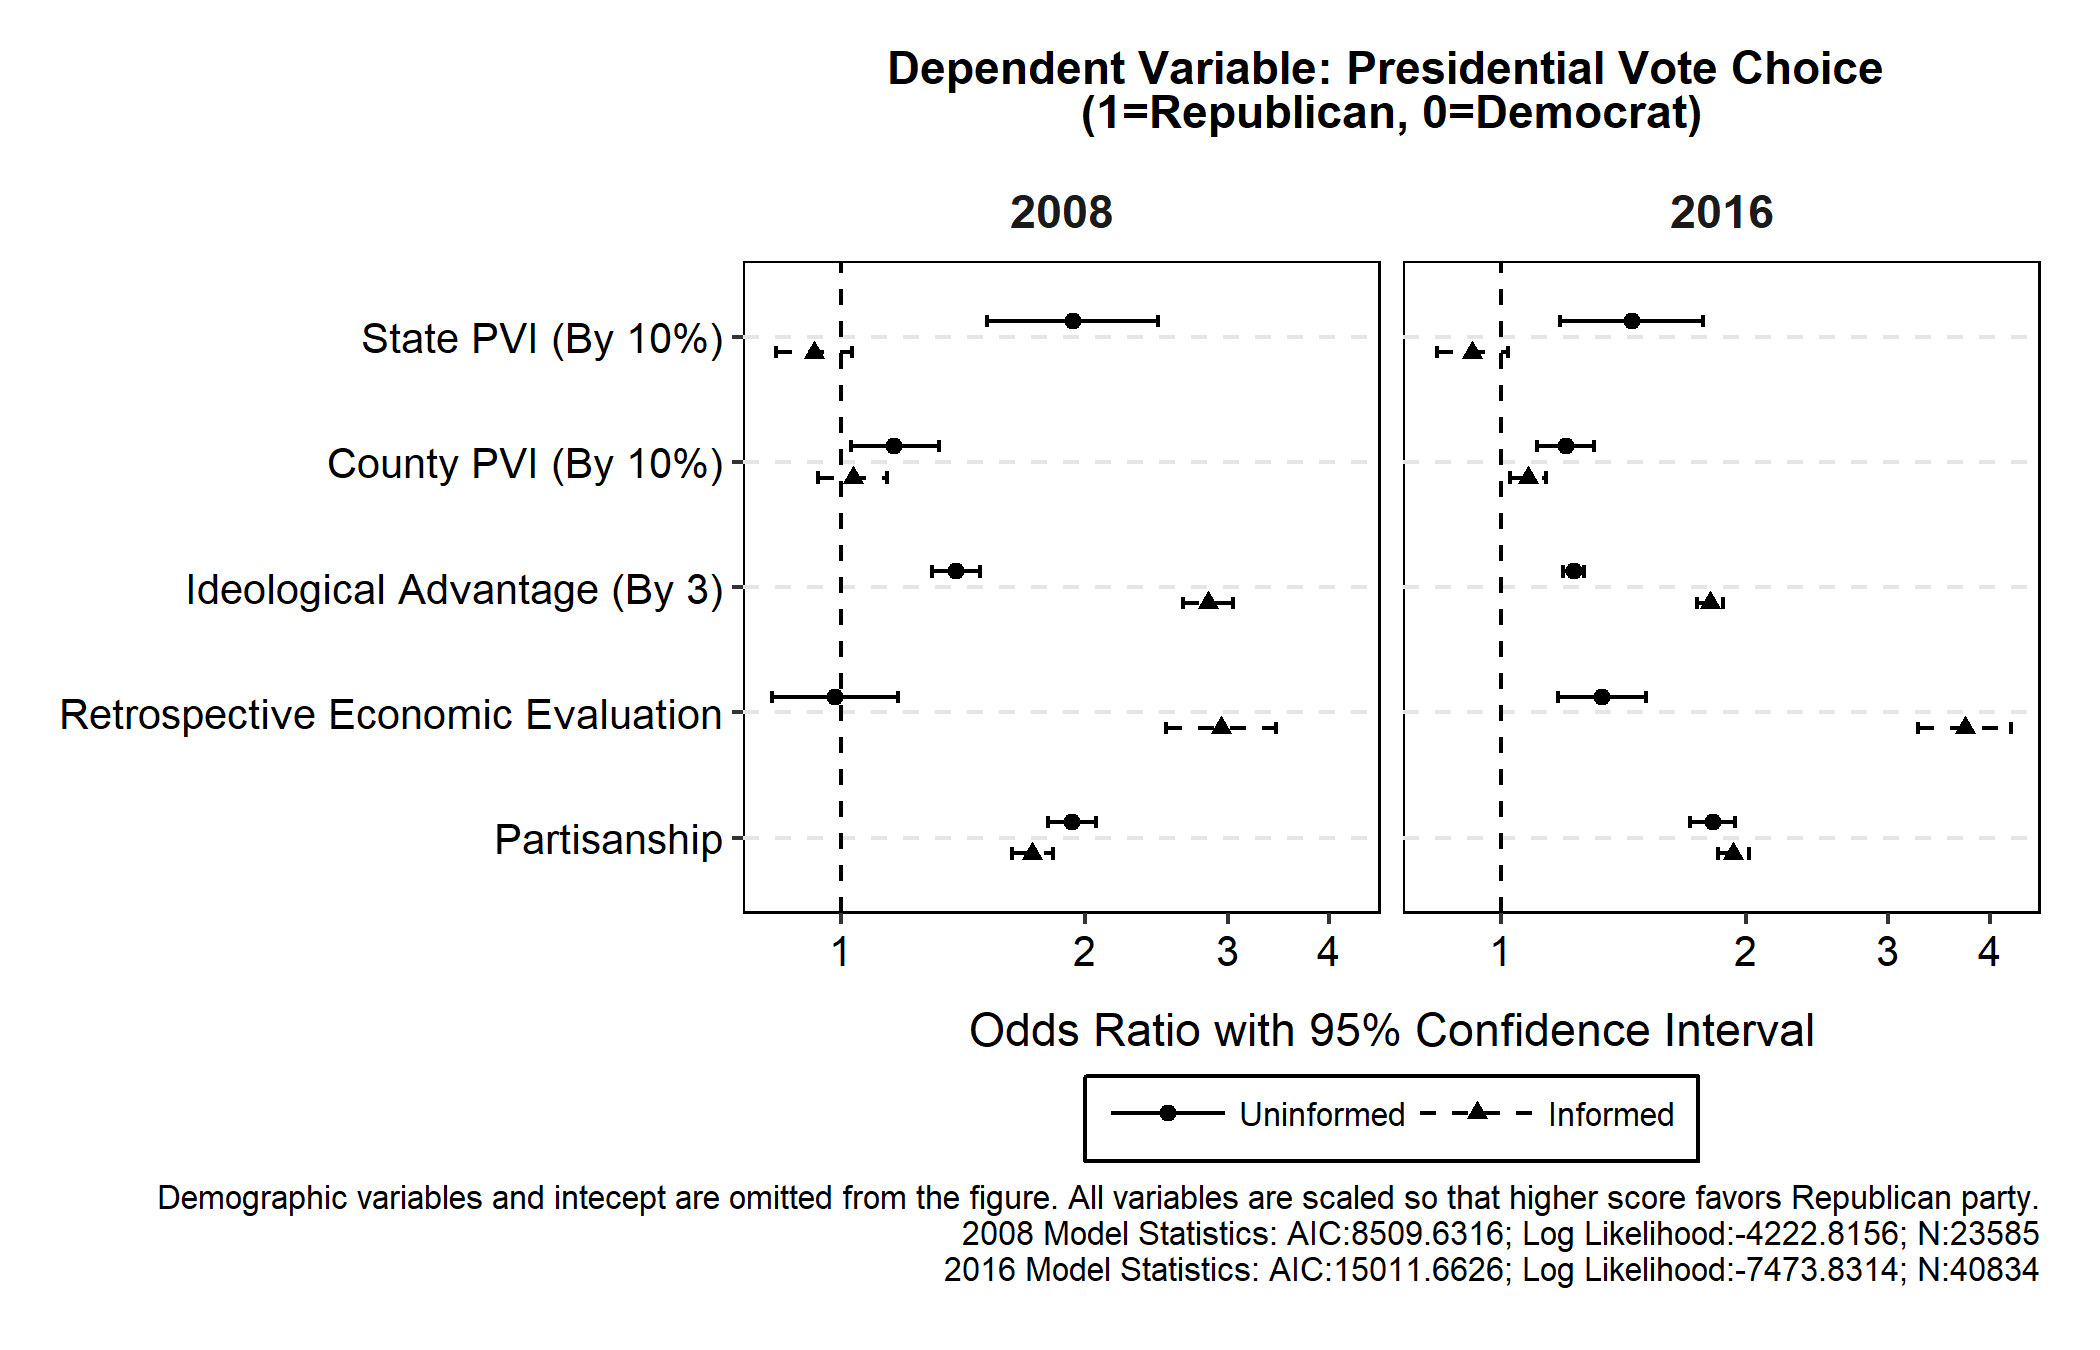
\includegraphics[width=\linewidth]{../outputs/ccescoefplot.png}
    \end{figure}

    \par The summary of presidential vote choice model is presented in \autoref{fig:ccescoefplot}. The figure shows conditional odds ratios for fully informed voters (political knowledge $= 1$) and uninformed voters (political knowledge $= 0$) with 95\% confidence intervals. The figure omits demographic variables and intercepts (see Online Appendix A). The first and second rows of the plot show the impact of the local partisan environment on voting behavior. Consistent with H2, the odds ratios of state and county PVI are larger for uninformed voters than for informed voters. All PVI coefficients for uninformed voters are statistically significant ($p<0.05$), while three out of four PVI coefficients for informed voters are not statistically significant ($p>0.05$). The result also gives consistent support of H3 (bandwagoning): By every 10\% movement in local PVI towards Republican, uninformed voters are 1.5 to 2 times (for state PVI), and 1.2 times (for county PVI) more likely to vote for Republican than Democrat.
    
    \par For individual preference variables, the result generally supports H1. Ideology and retrospective economic evaluation variables have significantly larger odds ratios for informed than for uninformed voters. The partisanship variable, on the other hand, has a similar level of power to explain vote choice among informed and uninformed voters. Uninformed voters do not rely on ideological preferences and retrospective evaluations while using party identity in a way similar to that of informed voters.
    
    \par To gain deeper understandings of results regarding contextual variables, I simulate the predicted probability of the Republican vote through the Monte Carlo method. Since the estimated model includes complex sets of interacted variables, the simulation takes two steps. First, I estimated the predicted probability of vote choice for each respondent in surveys by manipulating the values only of the local partisan environment (from 5th percentile to 95th percentile), and political knowledge ($0$ and $1$). Each prediction is made by drawing 1,000 random coefficients according to the multivariate normal distribution, with mean as a point estimate and clustered standard error. Second, I averaged predicted probabilities according to the population weight provided in CCES. This procedure gives the approximation of the average two-party Republican vote probability under the given local partisan environment and knowledge level.

    \begin{figure}[t!]
        \caption{Local partisan environments and average predicted probability of two-party Republican vote in CCES (2008, 2016)}
        \label{fig:ccespredplot}
        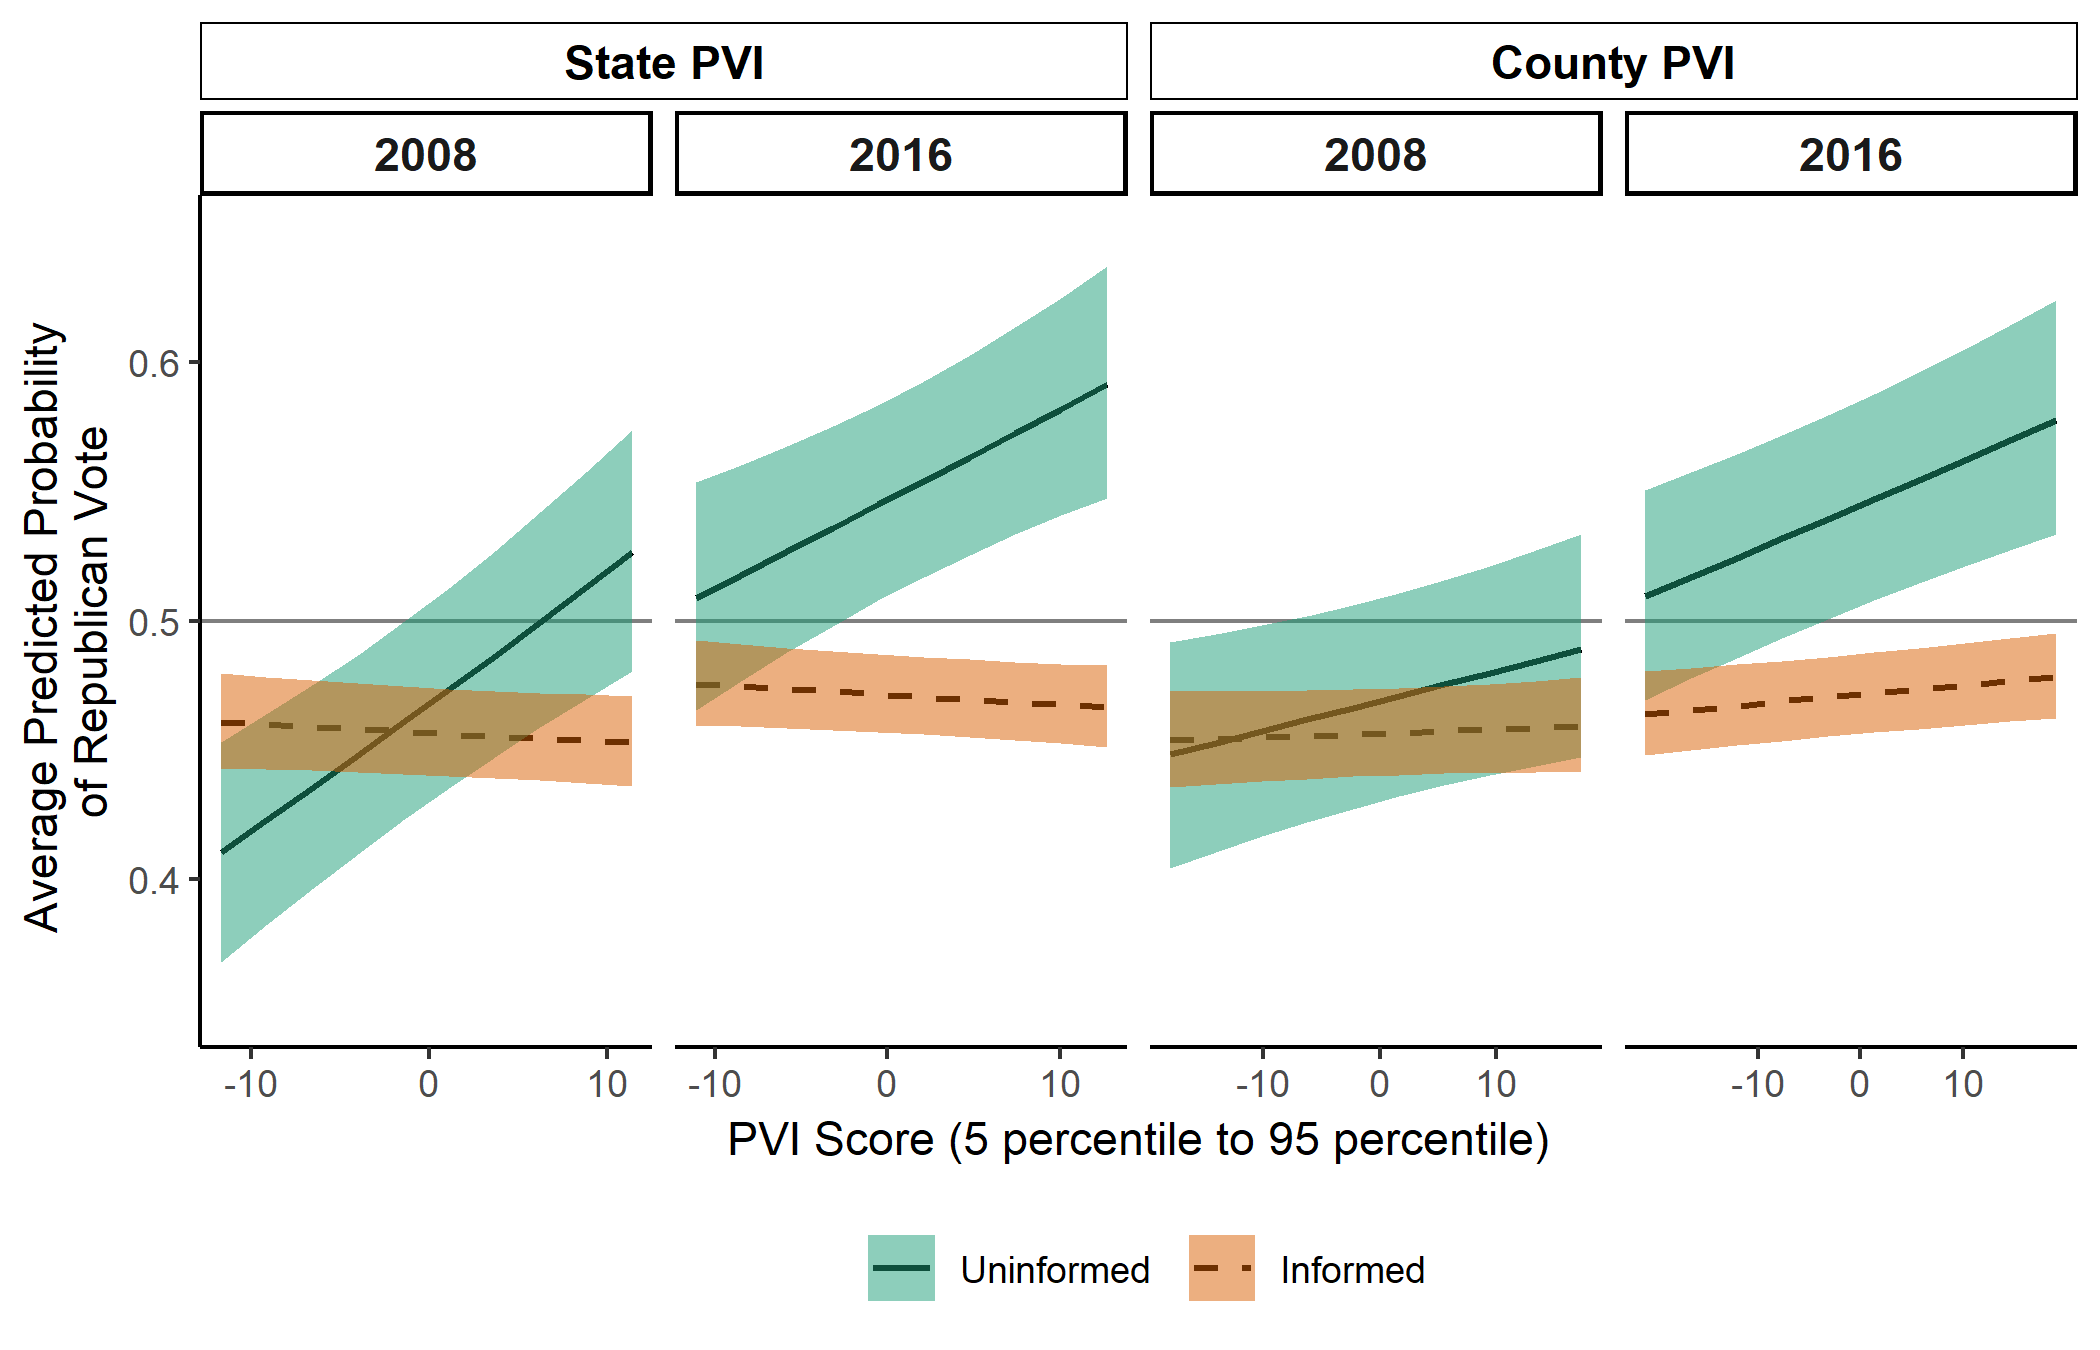
\includegraphics[width=\linewidth]{../outputs/ccespredplot.png}
    \end{figure}
        
    \par \autoref{fig:ccespredplot} plots the simulation result. The shaded area represents 95\% confidence intervals in prediction. Here, uninformed voters strongly respond to the local partisan environment, while informed voters don't.  Especially in 2016, the local partisan environment significantly raises the predicted vote probability of Trump among uninformed voters. The movement from the 5th percentile to the 95th percentile in state PVI and county PVI each correspond with a 10 to 13\% increase in Republican vote share. The impact of the local partisan environment in the 2008 election is somewhat weaker, but the predicted Republican vote probability for uninformed voters increase from $41.0$\% to $52.7$\% when the state PVI moves from and 11.7\% Democratic advantage (5th percentile) to an 11.4\% Republican advantage (95th percentile).
    
    \par The current study highlights the importance of the local partisan environment in explaining uninformed voting (but not informed voting). Uninformed voters show a clear tendency of bandwagoning: to vote in line with the majority in the local environment. Informed voters, on the other hand, rely mostly on their individual responses to make voting decisions and are unresponsive to the local partisan environment.

    \section*{Study 2: National Partisan Environment and Uninformed Voting}

    \par This section examines the relationship between the national partisan environment and voting choice in American presidential elections. I use the collection of data from American National Election Studies (ANES), conducted during presidential elections that occurred between 1972 and 2016.\footnote{I limit the analysis to respondents interviewed in face-to-face or phone mode. Online survey samples are dropped from the analysis due to comparability issues.} This dataset covers 12 presidential elections over a 44-year period, which reveals sufficient variations to assess the impact of the national partisan environment on uninformed voting. As in Study 1, the national partisan environment at each election is captured by the data obtained from CQ Press Voting and Election Collections. 

    \subsection*{Variables}
    
    \par The primary dependent variable for this study is the vote choice in presidential elections. As in Study 1, I focus on the binary choice between Republican and Democratic candidates and drop reported third-candidate choosers and abstainers from the analysis. The interviewer's rating of knowledge is used as the measure of \textit{political knowledge}. While this measure does not directly reflect the factual knowledge of respondents, it has a favorable quality to ensure comparability across surveys over time. The resultant measure is normalized to the range between 0 and 1, following the procedure that is taken by \cite{Bartels1996unvo}. The robustness check using the knowledge measure based on factual test questions yields similar results (see Online Appendix B).
    
    \par The measures of \textit{national partisan environment} are constructed in a way similar to those for the local partisan environment. Specifically, the national PVI uses the following formula for each election cycle $t$:
    \begin{align*}
        \textit{[National PVI]}_{t} = \{ & \textit{[National Republican Share]}_{t-1} + \\  
        &\textit{[National Republican Share]}_{t-2} \}/2
    \end{align*}
    \noindent \textit{National PVI} represents the national advantage of Republican party vote share over the Democratic party. The measure averages two previous elections to adjust for any short-term noise imposed during a single election cycle.
        
    \par In addition, \textit{individual preference} predictors (i.e., relative ideological advantage is based on squared distance from candidates, partisanship, and the retrospective economic evaluation) and \textit{demographic} controls (i.e., gender, age, race, income, education, and religion) are collected from each survey. All variables are scaled identically to the method used in Study 1 (see Online Appendix). 
        
    \subsection*{Model}

    \par In conducting the analysis, pooling all election years into one dataset over-complicates the model, because the distribution and the predictive power of voter characteristics may differ across elections. To cope with this heterogeneity, I follow a three-step procedure. First, the model of vote choice is constructed and estimated for each election year. As in Study 1 and \cite{Bartels1996unvo}, each model includes the complete set of interactions between political knowledge and all other covariates and estimated by the logistic regression with population weights provided for each survey.
    
    \par In the second step, following the procedure in Study 1, I simulated the weighted average of predicted probability of the Republican vote for fully informed (political knowledge $=1$) and uninformed voters (political knowledge $=0$). To control for the change in voter characteristics across years, the prediction is made by fixing the voter profiles to the specific election year. By fixing the voter profile, the simulation produces the prediction of how informed and uninformed voters would have voted in each election if the distribution of individual preferences and demographic characteristics stays constant. 
    
    \par Lastly, simulated Republican vote probabilities are regressed on the national partisan environment using the Estimated Dependent Variable (EDV) model \citep{Lewis2005esre, Kasara2015whdo}. The EDV model incorporates measurement uncertainty in the dependent variable, in the current case the vote probability estimate, in running OLS regression. This procedure allows both flexible modeling of vote choice in each election and controlling of the change in distributions of voter preferences and characteristics over the years.
    
    \subsection*{Results}

    \begin{figure}[t!]
        \caption{The impact of individual preferences on presidential vote vhoice in ANES (1972--2016)}
        \label{fig:anescoefplot}
        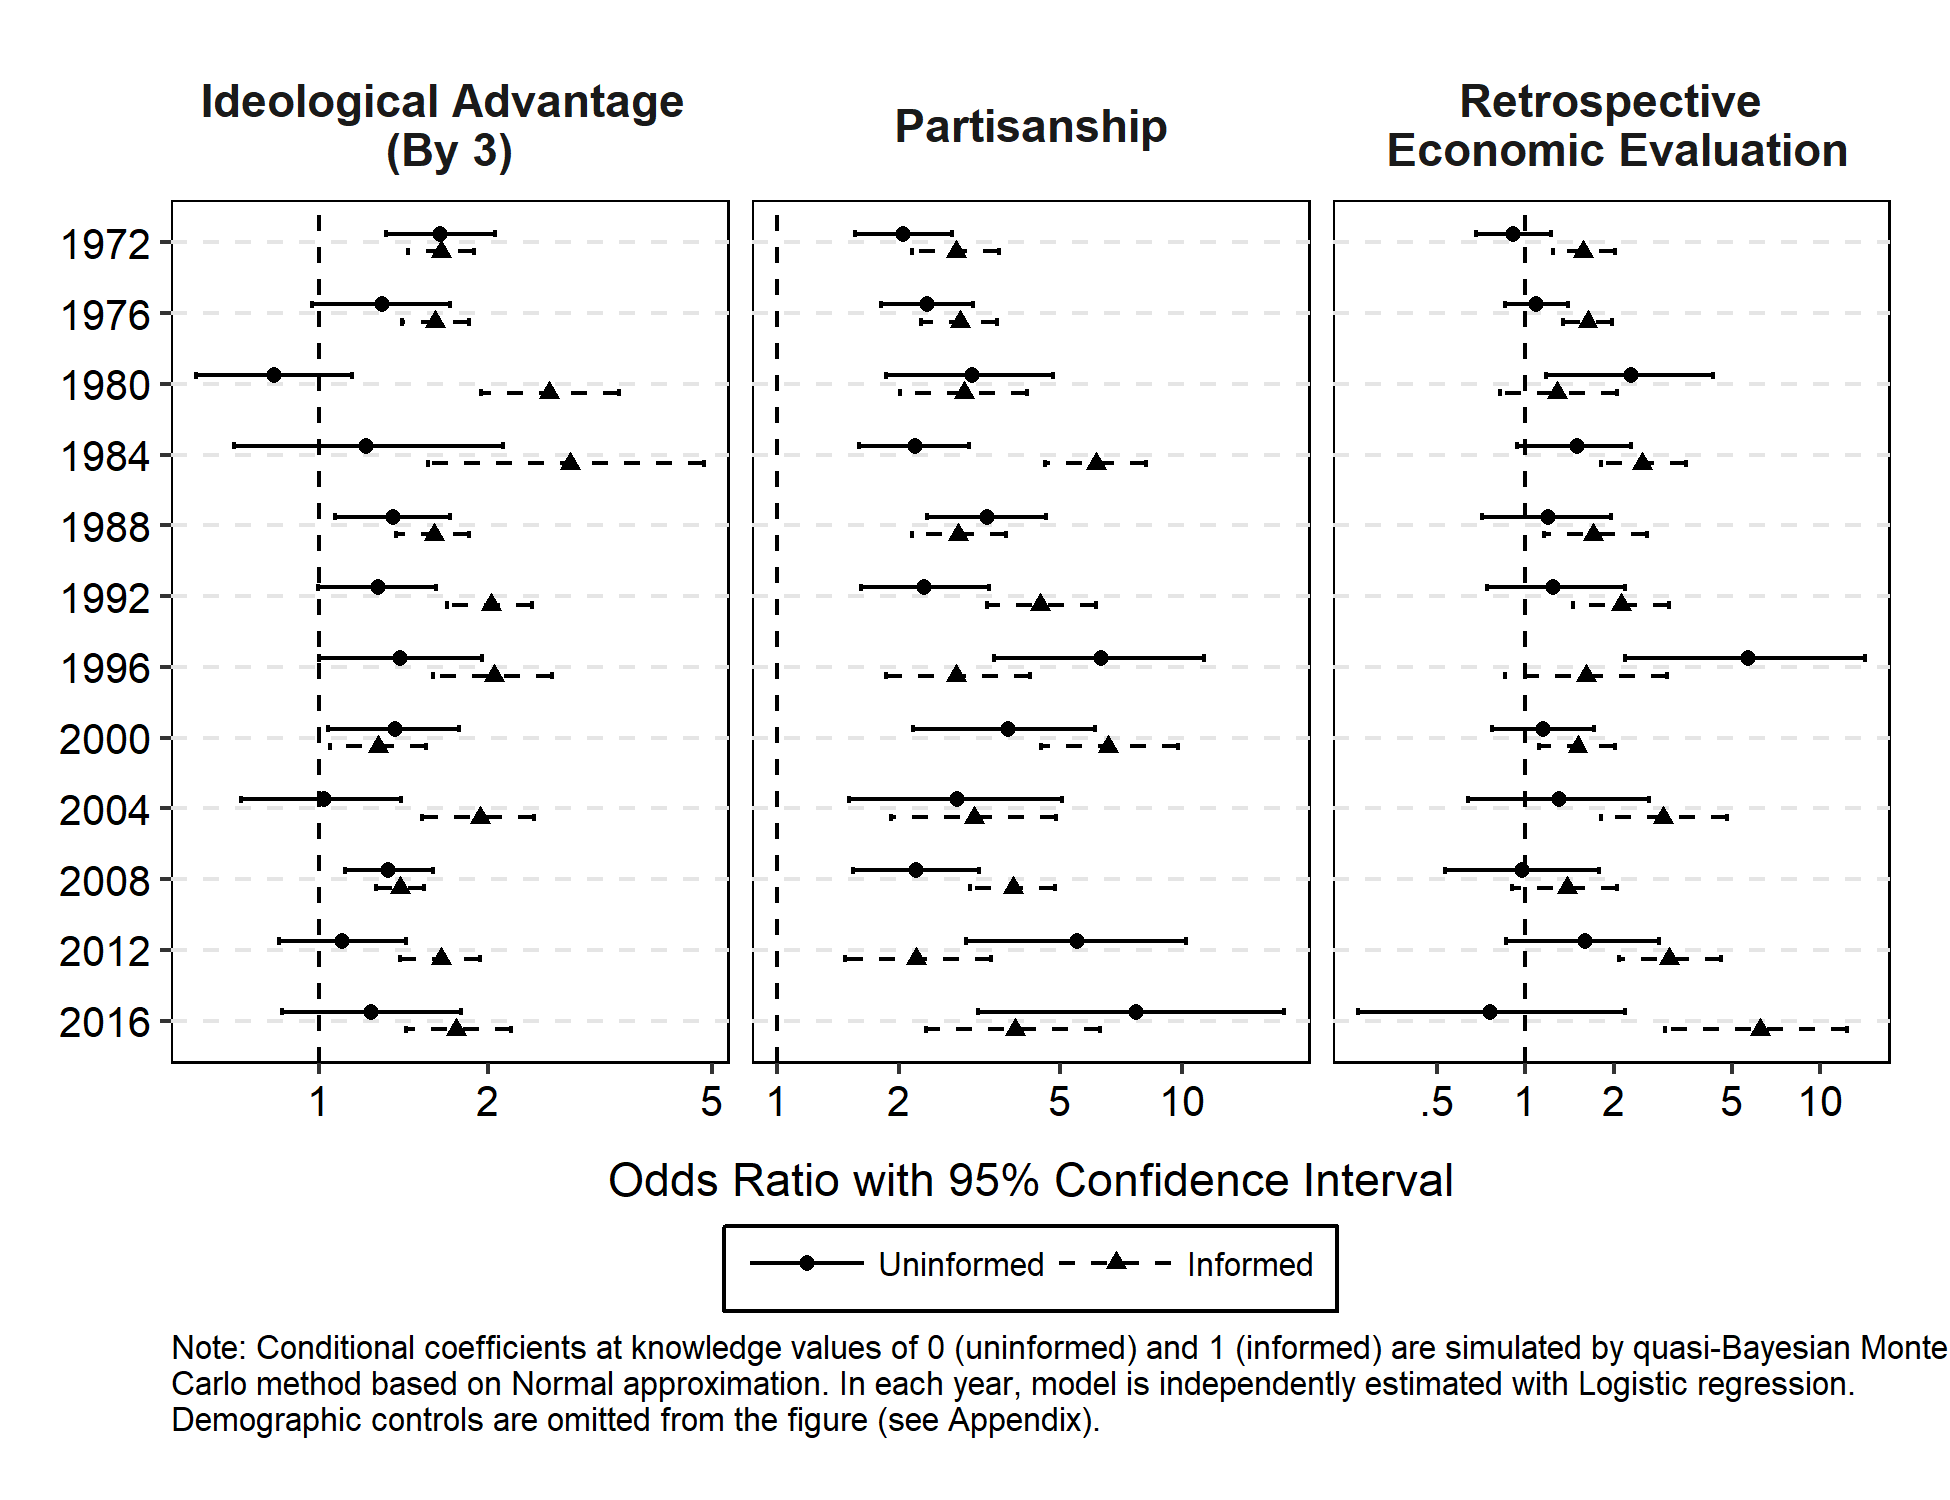
\includegraphics[width=\linewidth]{../outputs/m1sq_anescoefplot.png}
    \end{figure}

    \par \autoref{fig:anescoefplot} shows the conditional coefficients of individual preferences extracted from the vote choice models estimated in each election year. The results are consistent with the findings from Study 1, supporting H1 except for partisanship. The left panel indicates that the coefficient of ideological alignment is larger for informed voters than for uninformed voters in 11 out of 12 elections except for the year 2000. Similarly, the coefficient of retrospective economic evaluation (the right panel) is larger for informed voters than for uninformed voters in 10 out of 12 elections except for 1980 and 1996. On the other hand, the results on partisanship variables (the central panel) are mixed. Informed voters have larger coefficients in only seven elections, and uninformed voters have larger coefficients in five other elections.

    \par Following the described modeling procedure, \autoref{fig:anespredplot} presents the average predicted probabilities of Republican vote for fully informed (political knowledge $=1$) and uninformed (political knowledge $=0$) in each election year based on the 1992 voter profile. The voter profile from any given year yields similar results (see Online Appendix). 

    \begin{figure}[t!]
        \caption{National partisan environment and average predicted probability of two-party Republican vote in ANES (1972--2016)}
        \label{fig:anespredplot}
        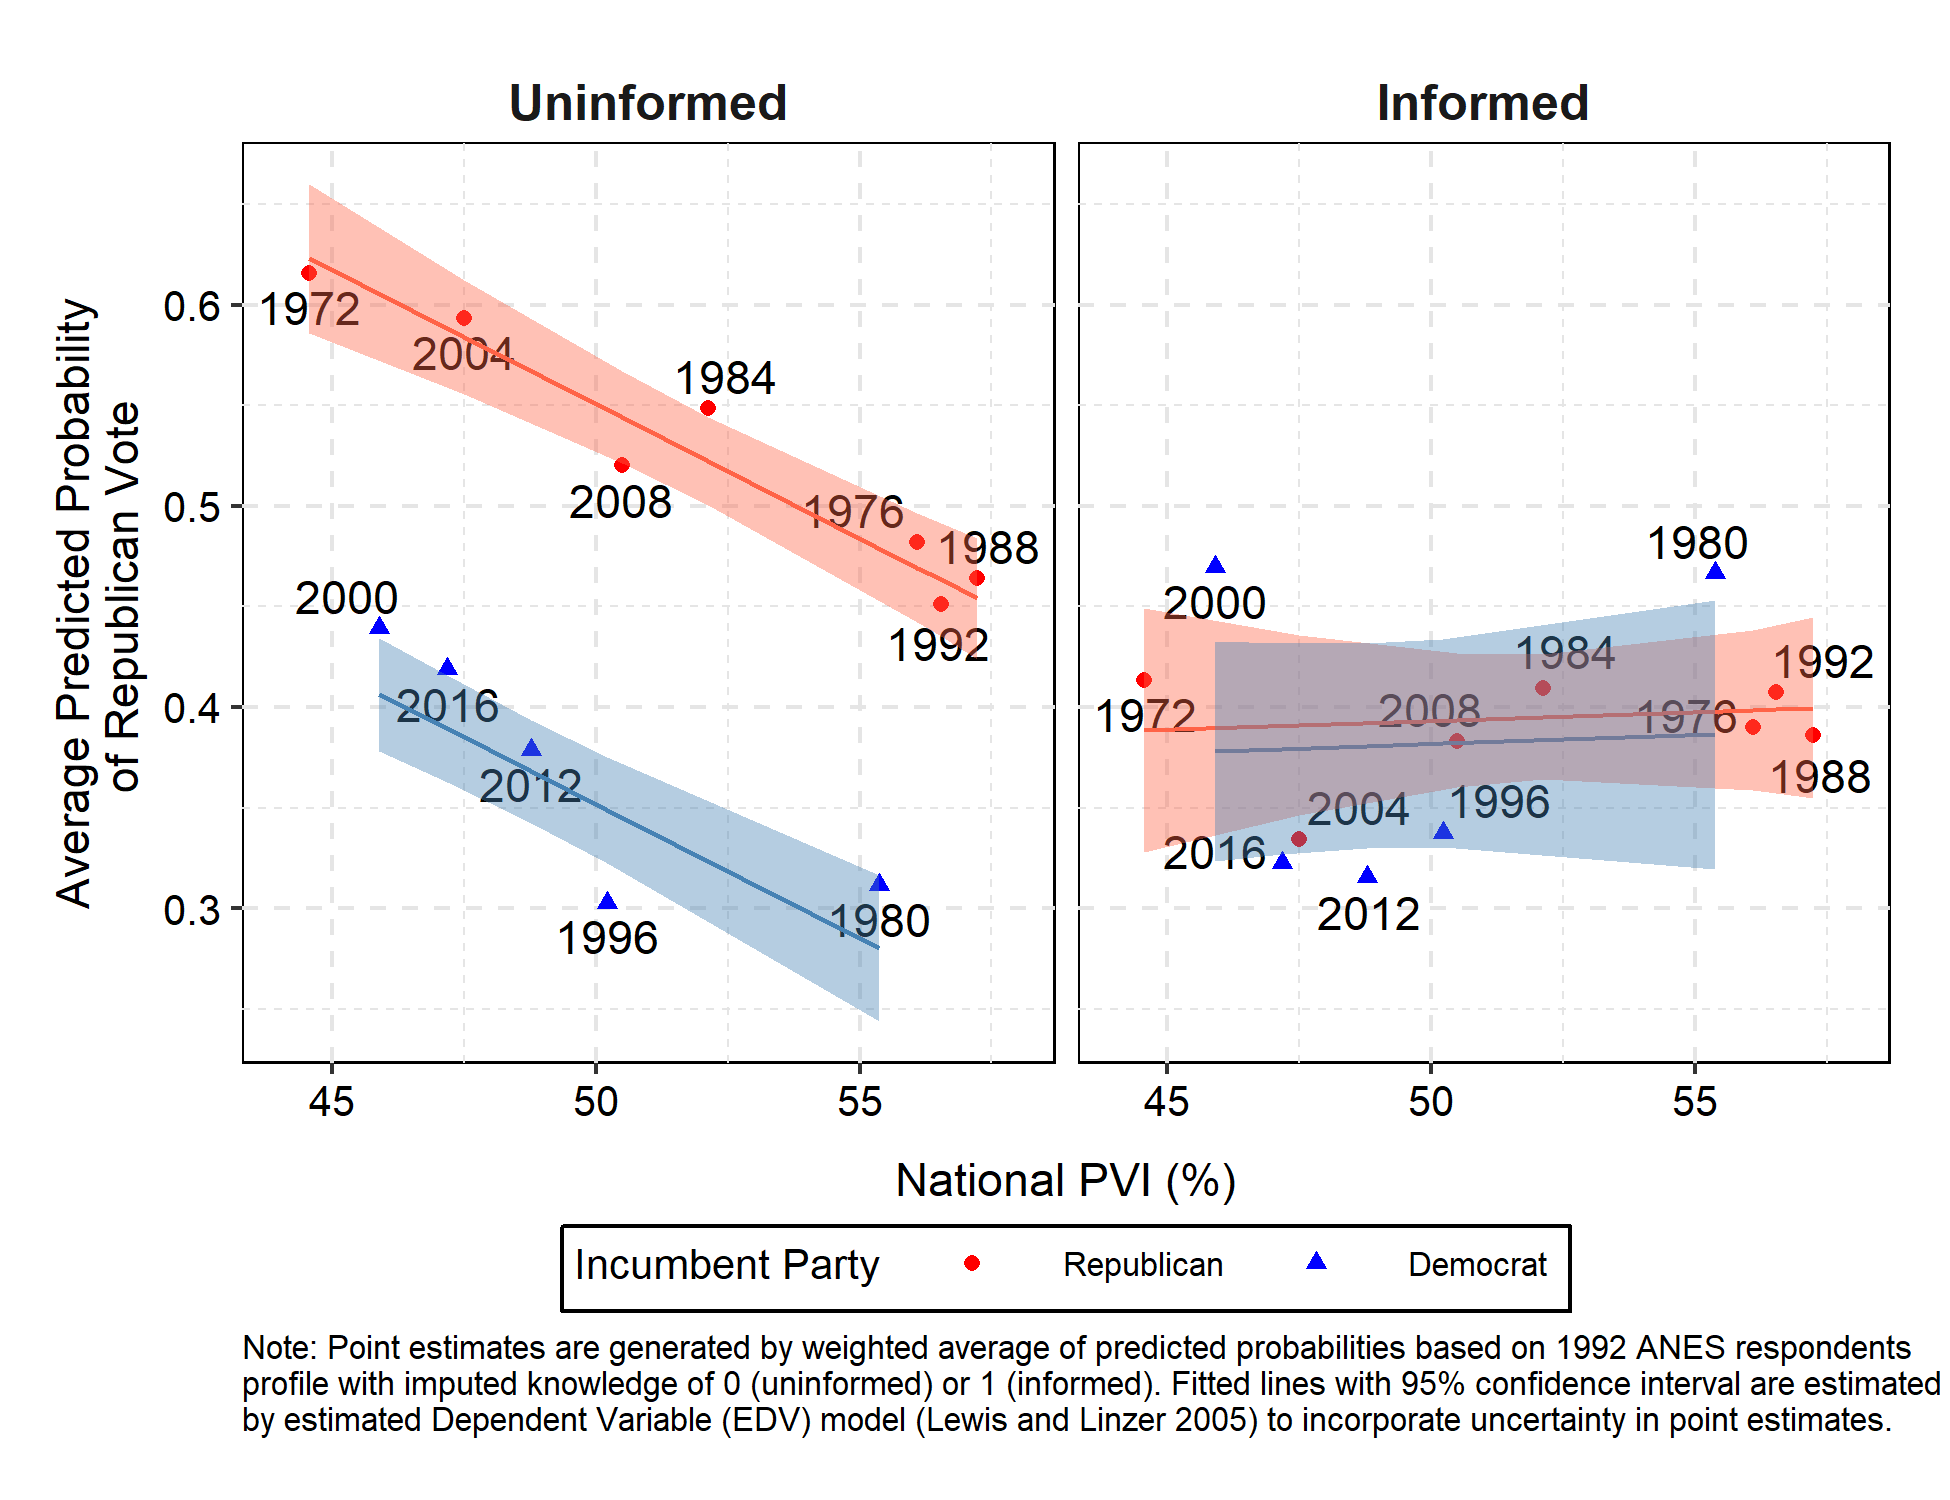
\includegraphics[width=\linewidth]{../outputs/m1sq_1992_anespredplot.png}
    \end{figure}

    \par The left panel of \autoref{fig:anespredplot} implies that the national-level pattern of uninformed voting is a function of two factors: the national partisan environment and the incumbent party. Uninformed voters favor the incumbent party but balance against the overly skewed national partisan environment. The left panel shows that after controlling for incumbent party, the stronger the partisan skew towards Republican (the higher the score of national PVI), the less likely uninformed voters are to vote for Republican candidates. The fitted lines with the 95\% confidence interval from the EDV regression show that two factors produce almost a perfect fit of the variations in average uninformed Republican vote probabilities. The right panel indicates that this pattern does not exist for informed voters: The average predicted probability of informed Republican votes are mostly unresponsive to the change in incumbent party and the national partisan environment.
    
    \section*{Discussion}
    
    \par Overall, the analysis suggests that local and national partisan environments play a crucial role in explaining the behavior of uninformed voters. While informed voting is dominated by individual preferences, uninformed voters bandwagon with the local partisan environment (Study 1) and balance against the national partisan environment (Study 2). The result of this study provides consistent evidence that informed and uninformed voters apply different logic in making vote choices. Especially, the evidence of balancing implies that uninformed voters have an incentive and an ability to vote strategically.
    
    \par This study offers clues to answer the question left in the empirical studies of information effects: \textit{Why} does information make a systematic difference in the outcome of voting choices? The partisan environment is one of the key variables to understand why informed and uninformed voters act in different ways. Using this result, the scholarly debate on civic competence can move forward instead of focusing on how illogical and unpredictable uninformed voters are, the conversation can shift to the exploration of how the logic of uninformed voting relates to the quality of democratic outcomes. 
    
    \par Three caveats remain. First, it is not clear if the findings can be generalized outside of the context of presidential elections under a two-party system. Further exploration of voting patterns under parliamentary and multi-party system is needed. Second, the measurement of the partisan environment has an issue of visibility. The objective measure used in this study does not ensure that this information is directly observed by the respondent. Further research should consider how the knowledge of the partisan environment is communicated to uninformed voters (e.g., social network and public opinion polls). Third, this study ignores the participation incentives of uninformed voters. Many studies suggest that political knowledge plays an important role in turnout decisions \citep{Matsusaka1995exvo, Dellicarpini1996wham, Feddersen1996thsw, Lassen2005thef, Larcinese2007dopo, Gemenis2014voad}. To fully grasp the picture of uninformed voting, one needs to take abstention incentives into account.
    
    \par Finally, one promising direction in which to extend the current analysis is exploration of the interactive nature of context-based uninformed voting. The recent developments in game theoretic and simulation research suggest that after accounting for the dynamic interaction process among voters or between voters and a policymaker, the lack of voter information is not crucial for, or even improving, the quality of democratic decisions \citep{Ashworth2014isvo, Couzin2011unin}. Exploring the implications of those interactions for context-based uninformed voting would be an important contribution to this line of inquiry. 
    
    %\clearpage
    % \theendnotes
    \singlespacing
    %\nocite{*}
    \bibliographystyle{apsr}
    % \bibliography{C:/GoogleDrive/Reference/list_jabref.bib}
    %\bibliography{/home/gentok/GoogleDrive/Reference/list_jabref.bib}
    \bibliography{uninformedchoice.bib}

    \clearpage
\appendix

\section*{Supporting Materials (Not Intended for Print)}

\par This is the Online Appendix of ``Local Bandwagoning and National Balancing: How Uninformed Voters Respond to Partisan Environments and Why It Matters.'' 

\section{Study 1 Appendix} \label{appA}
\setcounter{table}{0}
\renewcommand{\thetable}{A\arabic{table}}
\setcounter{figure}{0}
\renewcommand{\thefigure}{A\arabic{figure}}

\subsection{Variable Constructs} 

\par Knowledge variables in CCES datasets are constructed by aggregating correct answers from following eight questions. The final score is normalized to the 0-1 range: 0 indicates all incorrect, and 1 indicates all correct.

\begin{itemize}
    \item Majority party in the federal House (2008: \textit{CC308a}; 2016: \texttt{CC16\_321a})
    \item Majority party in the federal Senate (2008: \texttt{CC308b}; 2016: \texttt{CC16\_321b})
    \item Majority party in the state Senate (2008: \texttt{CC308c}; 2016: \texttt{CC16\_321c})
    \item Majority party in the state House (2008: \texttt{CC308d}; 2016: \texttt{CC16\_321d})
    \item The party of the federal House incumbent (2008: \texttt{CC309d}; 2016: \texttt{CC16\_322d})
    \item The party of the federal Senate incumbent 1 (2008: \texttt{CC309b}; 2016: \texttt{CC16\_322b})
    \item The party of the federal Senate incumbent 2 (2008: \texttt{CC309c}; 2016: \texttt{CC16\_322c})
    \item The party of the state governor incumbent (2008: \texttt{CC309a}; 2016: \texttt{CC16\_322a})
\end{itemize}

\begin{figure}[ht!!!]
    \caption{The distribution of political knowledge (CCES)}
    \label{fig:knidxgraph2}
    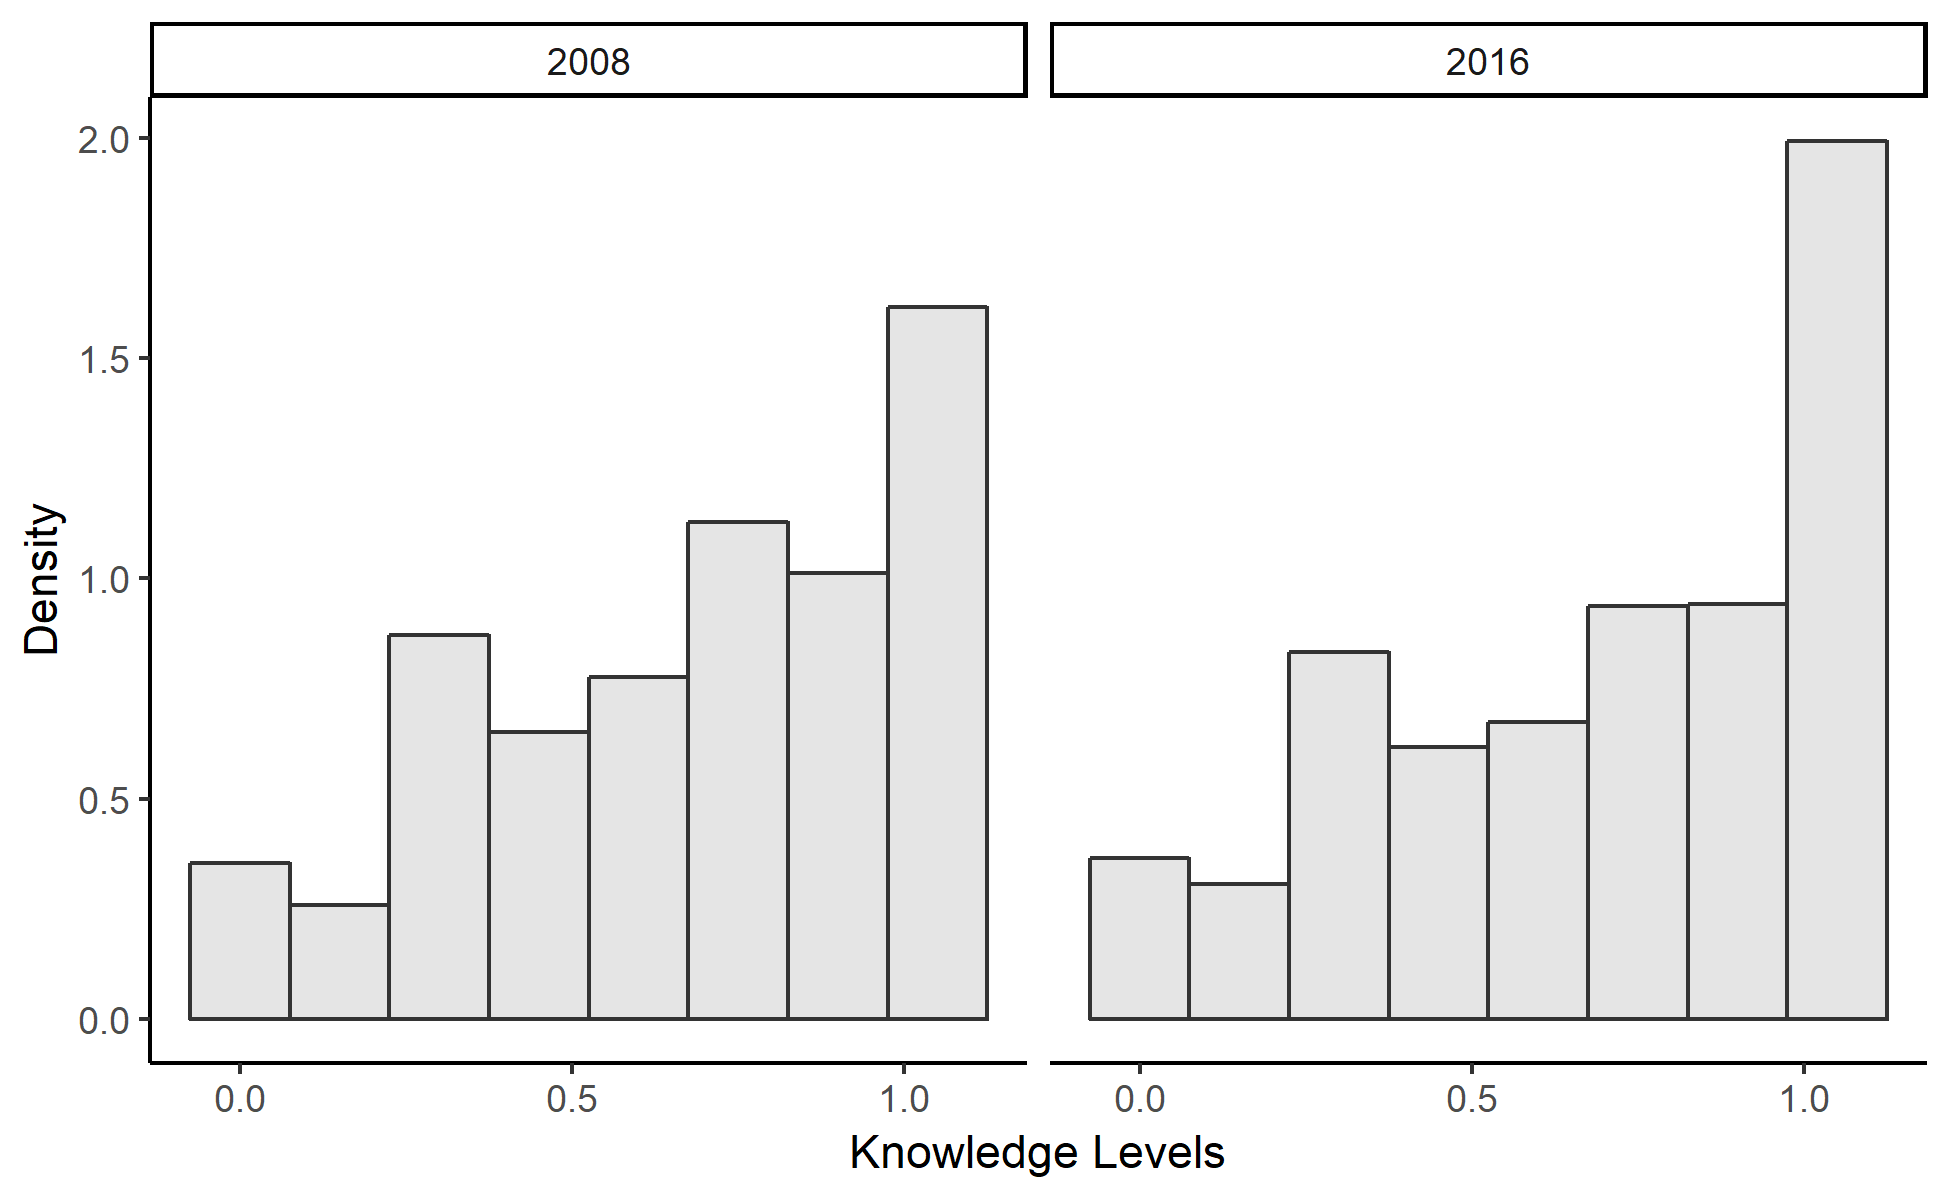
\includegraphics[width=\linewidth]{../outputs/cces_knowdist.png}
\end{figure}

\par \autoref{fig:knidxgraph2} shows the distribution of political knowledge in CCES datasets. It shows that the large portion of respondents are fully informed of the factual questions offered in the survey (political knowledge $= 1$), while there are significant numbers of respondents who are uninformed or only partially informed. The distribution of knowledge is similar across 2008 and 2016 elections, while the 2016 election involves slightly more informed respondents. Given the nature of CCES as the online survey, it should be cautioned that the absolute distribution of knowledge may not be representative of the voters in the actual election. For this study, it needed to be confirmed that there is a sufficient number of informed and uninformed voters to make a comparison of their behavioral patterns.

\begin{figure}[ht!!!]
    \caption{The distribution of local partisan environment (CCES)}
    \label{fig:pvigraph2}
    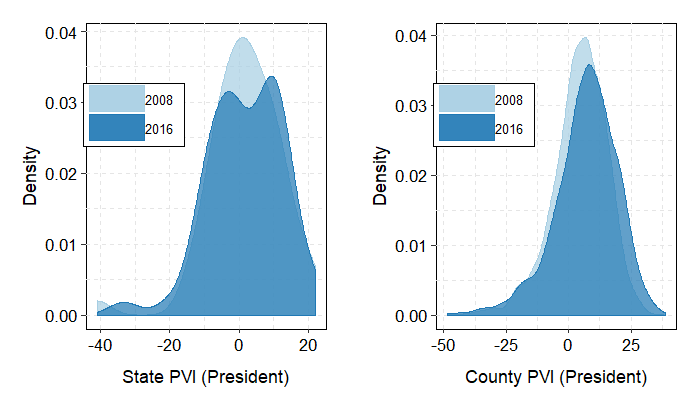
\includegraphics[width=\linewidth]{../outputs/cces_pvidist.png}
\end{figure}

\par Next, \autoref{fig:pvigraph2} shows the density distributions of local partisan environment variables. State level PVI is presented in the left-hand panel, and county level PVI is presented in right-hand panels. Those graphs show that the distributions of PVI are mostly single-peaked (with the slight exception in state PVI in 2016) and skewed to the left (there is a small number of units that are highly Democratic). It is also confirmed that significant variations exist in both state level and county level PVI. Even after adjusting for the state partisan environment, county level PVI still have a sufficient variance to explain vote choice. In fact, looking at the range of values in PVI, county PVI has a wider spread than state PVI.

\par Other variables are constructed from the following questions in CCES dataset:

\begin{itemize}
    \item Presidential vote choice (2008: \texttt{CC403} and \texttt{CC410}; 2016: \texttt{votereg\_post}, \texttt{CC16\_401} and \texttt{CC16\_410a}). 1 is voting for Republican, 0 is voting for Democrat. All other responses are dropped from the analysis.
    \item Republican advantage in squared ideological distance. Constructed from respondent's self ideology location (2008: \texttt{CC317a}; 2016: \texttt{CC16\_340a}), Republican candidate's perceived ideological location (2008: \texttt{CC317g}; 2016: \texttt{CC16\_340e}), and Democratic candidate's perceived ideological location (2008: \texttt{CC317h}; 2016: \texttt{CC16\_340d}). Each ideological position variable is rescaled in -3 to 3 range (higher score indicates more Conservative). The final variable is scaled from -36 to 36 (higher score indicates that perceived ideological position of Republican candidate is closer than the perceived ideological position of Democratic candidate to self ideology position).
    \item The retrospective evaluation of national economy (2008: \texttt{CC302}; 2016: \texttt{CC16\_302}). In 2008, the variable is scaled from gotten much worse (-2) to gotten much better (2). ``Not sure'' is recoded to 0. The scale in 2016 is reverse scaled so higher score advantages Republican candidate.   
    \item Party identity (2008: \texttt{CC307a}; 2016: \texttt{pid7}). Scaled from strong Democrat (-3) to strong Republican (3). ``Not sure'' is recoded to 0.
    \item Gender (2008: \texttt{V208}; 2016: \texttt{gender}). 1 is female and 0 is male.
    \item Age (2008: \texttt{V207}; 2016: \texttt{birthyr}).
    \item Race (2008: \texttt{V211}; 2016: \texttt{race}). Dummy variables are created for White, Black, Latino, Asian, and other races.
    \item Family income (2008: \texttt{V246}; 2016: \texttt{faminc}).
    \item Education (2008: \texttt{V213}; 2016: \texttt{educ}).
    \item Born-again Christian (2008: \texttt{V215}; 2016: \texttt{pew\_bornagain}).
\end{itemize}

\clearpage
\subsection{Detailed Logistic Regression Tables} 

\par Following tables show the full set of models estimated in CCES dataset. For both 2008 and 2016, Model 3 is used as the final model presented in the main text.

\begin{table}[ht!!!]
    \footnotesize
    \centering
    \caption{2008 Presidential Vote Choice (CCES: Republican=1, Democrat=0)}
    
\begin{tabular}{l D{)}{)}{13)3} D{)}{)}{13)3} D{)}{)}{13)3} }
\toprule
 & \multicolumn{1}{c}{Model 1} & \multicolumn{1}{c}{Model 2} & \multicolumn{1}{c}{Model 3} \\
\midrule
(Intercept)                        & -0.913 \; (0.088)^{***} & -0.423 \; (0.188)^{*}   & -0.169 \; (0.707)       \\
Knowledge                          & 1.040 \; (0.103)^{***}  & 1.054 \; (0.296)^{***}  & -0.030 \; (0.949)       \\
State PVI (By 10\%)                & 0.730 \; (0.100)^{***}  & 0.720 \; (0.121)^{***}  & 0.655 \; (0.148)^{***}  \\
County PVI (By 10\%)               & 0.435 \; (0.059)^{***}  & 0.346 \; (0.088)^{***}  & 0.149 \; (0.076)^{*}    \\
Knowledge*State PVI                & -0.481 \; (0.117)^{***} & -0.746 \; (0.160)^{***} & -0.735 \; (0.186)^{***} \\
Knowledge*County PVI               & -0.020 \; (0.065)       & -0.224 \; (0.136)       & -0.114 \; (0.115)       \\
Ideological Advantage              &                         & 0.107 \; (0.014)^{***}  & 0.108 \; (0.014)^{***}  \\
Retrospective Economic Evaluation  &                         & -0.117 \; (0.116)       & -0.021 \; (0.110)       \\
Partisanship                       &                         & 0.721 \; (0.046)^{***}  & 0.654 \; (0.042)^{***}  \\
Knowledge*Ideological Advantage    &                         & 0.233 \; (0.020)^{***}  & 0.239 \; (0.021)^{***}  \\
Knowledge*Retrospective Evaluation &                         & 1.090 \; (0.186)^{***}  & 1.100 \; (0.183)^{***}  \\
Knowledge*Partisanship             &                         & -0.189 \; (0.063)^{**}  & -0.111 \; (0.064)       \\
Female                             &                         &                         & 0.005 \; (0.150)        \\
Age                                &                         &                         & -0.958 \; (2.959)       \\
Age Squared                        &                         &                         & 2.876 \; (3.349)        \\
Black                              &                         &                         & -5.093 \; (0.915)^{***} \\
Latino                             &                         &                         & -1.190 \; (0.298)^{***} \\
Asian                              &                         &                         & -0.254 \; (0.620)       \\
Other Race                         &                         &                         & -1.256 \; (0.423)^{**}  \\
Income                             &                         &                         & 0.305 \; (0.370)        \\
Education                          &                         &                         & -0.635 \; (0.351)       \\
Born-Again Christian               &                         &                         & 0.473 \; (0.177)^{**}   \\
Knowledge*Female                   &                         &                         & 0.621 \; (0.229)^{**}   \\
Knowledge*Age                      &                         &                         & 4.859 \; (4.131)        \\
Knowledge*Age Squared              &                         &                         & -5.714 \; (4.670)       \\
Knowledge*Black                    &                         &                         & 2.708 \; (1.191)^{*}    \\
Knowledge*Latino                   &                         &                         & 1.263 \; (0.494)^{*}    \\
Knowledge*Asian                    &                         &                         & -0.626 \; (1.015)       \\
Knowledge*Other Race               &                         &                         & 1.833 \; (0.524)^{***}  \\
Knowledge*Income                   &                         &                         & -0.335 \; (0.569)       \\
Knowledge*Education                &                         &                         & -0.032 \; (0.481)       \\
Knowledge*Born-Again Christian     &                         &                         & -0.185 \; (0.217)       \\
\midrule
AIC                                & 35422.565               & 9284.096                & 8509.631                \\
BIC                                & 35470.975               & 9380.916                & 8767.819                \\
Log Likelihood                     & -17705.283              & -4630.048               & -4222.816               \\
Deviance                           & 28030.919               & 7734.934                & 6961.932                \\
Num. obs.                          & 23585                   & 23585                   & 23585                   \\
\bottomrule
\multicolumn{4}{l}{\scriptsize{$^{***}p<0.001$, $^{**}p<0.01$, $^*p<0.05$}}
\end{tabular}

\end{table}

\begin{table}[ht!!!]
    \footnotesize
    \centering
    \caption{2016 Presidential Vote Choice (CCES: Republican=1, Democrat=0)}
    
\begin{tabular}{l D{)}{)}{13)3} D{)}{)}{13)3} D{)}{)}{13)3} }
\toprule
 & \multicolumn{1}{c}{Model 1} & \multicolumn{1}{c}{Model 2} & \multicolumn{1}{c}{Model 3} \\
\midrule
(Intercept)                        & -0.117 \; (0.099)      & 0.237 \; (0.104)^{*}    & -0.180 \; (0.588)       \\
Knowledge                          & 0.093 \; (0.102)       & -1.098 \; (0.139)^{***} & -0.512 \; (0.931)       \\
State PVI (By 10\%)                & 0.537 \; (0.117)^{***} & 0.425 \; (0.133)^{**}   & 0.374 \; (0.123)^{**}   \\
County PVI (By 10\%)               & 0.461 \; (0.041)^{***} & 0.331 \; (0.045)^{***}  & 0.183 \; (0.050)^{***}  \\
Knowledge*State PVI                & -0.146 \; (0.118)      & -0.479 \; (0.163)^{**}  & -0.458 \; (0.159)^{**}  \\
Knowledge*County PVI               & -0.089 \; (0.046)      & -0.185 \; (0.059)^{**}  & -0.105 \; (0.064)       \\
Ideological Alignment              &                        & 0.067 \; (0.006)^{***}  & 0.069 \; (0.006)^{***}  \\
Partisanship                       &                        & 0.662 \; (0.041)^{***}  & 0.601 \; (0.039)^{***}  \\
Retrospective Economic Evaluation  &                        & 0.246 \; (0.081)^{**}   & 0.286 \; (0.076)^{***}  \\
Knowledge*Ideological Alignment    &                        & 0.133 \; (0.010)^{***}  & 0.128 \; (0.009)^{***}  \\
Knowledge*Partisanship             &                        & 0.017 \; (0.054)        & 0.058 \; (0.052)        \\
Knowledge*Retrospective Evaluation &                        & 1.052 \; (0.112)^{***}  & 1.030 \; (0.121)^{***}  \\
Female                             &                        &                         & -0.849 \; (0.126)^{***} \\
Age                                &                        &                         & 5.086 \; (2.667)        \\
Age Squared                        &                        &                         & -4.982 \; (2.736)       \\
Black                              &                        &                         & -2.081 \; (0.350)^{***} \\
Latino                             &                        &                         & -1.388 \; (0.316)^{***} \\
Asian                              &                        &                         & -1.092 \; (0.316)^{***} \\
Other Race                         &                        &                         & -0.948 \; (0.243)^{***} \\
Income                             &                        &                         & 1.252 \; (0.352)^{***}  \\
Education                          &                        &                         & -0.832 \; (0.247)^{***} \\
Born-Again Christian               &                        &                         & 0.723 \; (0.141)^{***}  \\
Knowledge*Female                   &                        &                         & 0.385 \; (0.189)^{*}    \\
Knowledge*Age                      &                        &                         & -2.394 \; (3.715)       \\
Knowledge*Age Squared              &                        &                         & 2.170 \; (3.615)        \\
Knowledge*Black                    &                        &                         & 0.579 \; (0.655)        \\
Knowledge*Latino                   &                        &                         & 0.894 \; (0.758)        \\
Knowledge*Asian                    &                        &                         & 0.805 \; (0.413)        \\
Knowledge*Other Race               &                        &                         & 0.948 \; (0.399)^{*}    \\
Knowledge*Income                   &                        &                         & -1.399 \; (0.470)^{**}  \\
Knowledge*Education                &                        &                         & 0.008 \; (0.333)        \\
Knowledge*Born-Again Christian     &                        &                         & -0.379 \; (0.167)^{*}   \\
\midrule
AIC                                & 54029.263              & 15960.343               & 15024.881               \\
BIC                                & 54080.967              & 16063.750               & 15300.633               \\
Log Likelihood                     & -27008.632             & -7968.171               & -7480.440               \\
Deviance                           & 53681.964              & 16082.617               & 15075.333               \\
Num. obs.                          & 40834                  & 40834                   & 40834                   \\
\bottomrule
\multicolumn{4}{l}{\scriptsize{$^{***}p<0.001$, $^{**}p<0.01$, $^*p<0.05$}}
\end{tabular}

\end{table}

\clearpage
\subsection{Mixed Effects Logistic Regression} 

\par Following tables show the full set of models estimated in CCES dataset. All models are estimated by \texttt{glmer()} function from \texttt{lme4} R package with counties and states random effects.

\begin{table}[ht!!!]
    \footnotesize
    \centering
    \caption{2008 Presidential Vote Choice (CCES: Republican=1, Democrat=0)}
    
\begin{tabular}{l D{)}{)}{11)3} D{)}{)}{11)3} D{)}{)}{11)3} }
\toprule
 & \multicolumn{1}{c}{Model 1} & \multicolumn{1}{c}{Model 2} & \multicolumn{1}{c}{Model 3} \\
\midrule
(Intercept)                                 & -0.95 \; (0.05)^{***} & -0.41 \; (0.15)^{**}  & -0.05 \; (0.47)       \\
Knowledge                                   & 1.13 \; (0.05)^{***}  & 1.08 \; (0.24)^{***}  & -0.23 \; (0.77)       \\
State PVI (By 10\%)                         & 0.77 \; (0.07)^{***}  & 0.79 \; (0.11)^{***}  & 0.70 \; (0.11)^{***}  \\
County PVI (By 10\%)                        & 0.46 \; (0.04)^{***}  & 0.36 \; (0.06)^{***}  & 0.16 \; (0.07)^{*}    \\
Knowledge*State PVI                         & -0.52 \; (0.07)^{***} & -0.79 \; (0.13)^{***} & -0.76 \; (0.14)^{***} \\
Knowledge*County PVI                        & -0.06 \; (0.05)       & -0.25 \; (0.09)^{**}  & -0.13 \; (0.10)       \\
Ideological Advantage                       &                       & 0.11 \; (0.01)^{***}  & 0.11 \; (0.01)^{***}  \\
Retrospective Economic Evaluation           &                       & -0.09 \; (0.08)       & -0.02 \; (0.09)       \\
Partisanship                                &                       & 0.73 \; (0.03)^{***}  & 0.65 \; (0.04)^{***}  \\
Knowledge*Ideological Advantage             &                       & 0.24 \; (0.02)^{***}  & 0.24 \; (0.02)^{***}  \\
Knowledge*Retrospective Economic Evaluation &                       & 1.07 \; (0.14)^{***}  & 1.11 \; (0.15)^{***}  \\
Knowledge*Partisanship                      &                       & -0.17 \; (0.06)^{**}  & -0.09 \; (0.06)       \\
Female                                      &                       &                       & 0.01 \; (0.14)        \\
Age                                         &                       &                       & -0.20 \; (0.22)       \\
Age Squared                                 &                       &                       & 3.76 \; (2.41)        \\
Black                                       &                       &                       & -5.17 \; (0.59)^{***} \\
Latino                                      &                       &                       & -1.20 \; (0.22)^{***} \\
Asian                                       &                       &                       & -0.30 \; (0.51)       \\
Other Race                                  &                       &                       & -1.22 \; (0.38)^{**}  \\
Income                                      &                       &                       & 0.47 \; (0.32)        \\
Education                                   &                       &                       & -0.62 \; (0.27)^{*}   \\
Born-Again Christian                        &                       &                       & 0.46 \; (0.13)^{***}  \\
Knowledge*Female                            &                       &                       & 0.63 \; (0.22)^{**}   \\
Knowledge*Age                               &                       &                       & 0.62 \; (0.35)        \\
Knowledge*Age Squared                       &                       &                       & -6.89 \; (3.70)       \\
Knowledge*Black                             &                       &                       & 2.80 \; (0.82)^{***}  \\
Knowledge*Latino                            &                       &                       & 1.19 \; (0.37)^{**}   \\
Knowledge*Asian                             &                       &                       & -0.54 \; (0.84)       \\
Knowledge*Other Race                        &                       &                       & 1.84 \; (0.60)^{**}   \\
Knowledge*Income                            &                       &                       & -0.48 \; (0.51)       \\
Knowledge*Education                         &                       &                       & -0.10 \; (0.39)       \\
Knowledge*Born-Again Christian              &                       &                       & -0.16 \; (0.22)       \\
\midrule
AIC                                         & 27836.64              & 7648.86               & 6957.50               \\
BIC                                         & 27901.19              & 7761.82               & 7231.83               \\
Log Likelihood                              & -13910.32             & -3810.43              & -3444.75              \\
Num. obs.                                   & 23585                 & 23585                 & 23585                 \\
Num. groups: county                         & 2333                  & 2333                  & 2333                  \\
Num. groups: state                          & 51                    & 51                    & 51                    \\
Var: county (Intercept)                     & 0.12                  & 0.37                  & 0.28                  \\
Var: state (Intercept)                      & 0.04                  & 0.13                  & 0.10                  \\
\bottomrule
\multicolumn{4}{l}{\scriptsize{$^{***}p<0.001$, $^{**}p<0.01$, $^*p<0.05$}}
\end{tabular}

\end{table}

\begin{table}[ht!!!]
    \footnotesize
    \centering
    \caption{2016 Presidential Vote Choice (CCES: Republican=1, Democrat=0)}
    
\begin{tabular}{l D{)}{)}{11)3} D{)}{)}{11)3} D{)}{)}{11)3} }
\toprule
 & \multicolumn{1}{c}{Model 1} & \multicolumn{1}{c}{Model 2} & \multicolumn{1}{c}{Model 3} \\
\midrule
(Intercept)                                 & -0.06 \; (0.04)      & 0.29 \; (0.06)^{***}  & -0.14 \; (0.37)       \\
Knowledge                                   & 0.14 \; (0.04)^{***} & -1.13 \; (0.07)^{***} & -0.61 \; (0.59)       \\
State PVI (By 10\%)                         & 0.56 \; (0.05)^{***} & 0.48 \; (0.07)^{***}  & 0.42 \; (0.06)^{***}  \\
County PVI (By 10\%)                        & 0.44 \; (0.03)^{***} & 0.32 \; (0.04)^{***}  & 0.19 \; (0.04)^{***}  \\
Knowledge*State PVI                         & -0.15 \; (0.05)^{**} & -0.48 \; (0.08)^{***} & -0.46 \; (0.09)^{***} \\
Knowledge*County PVI                        & -0.08 \; (0.03)^{*}  & -0.16 \; (0.06)^{**}  & -0.09 \; (0.06)       \\
Ideological Advantage                       &                      & 0.07 \; (0.01)^{***}  & 0.07 \; (0.01)^{***}  \\
Retrospective Economic Evaluation           &                      & 0.22 \; (0.05)^{***}  & 0.28 \; (0.05)^{***}  \\
Partisanship                                &                      & 0.68 \; (0.03)^{***}  & 0.62 \; (0.03)^{***}  \\
Knowledge*Ideological Advantage             &                      & 0.13 \; (0.01)^{***}  & 0.13 \; (0.01)^{***}  \\
Knowledge*Retrospective Economic Evaluation &                      & 1.11 \; (0.07)^{***}  & 1.06 \; (0.08)^{***}  \\
Knowledge*Partisanship                      &                      & 0.02 \; (0.04)        & 0.05 \; (0.04)        \\
Female                                      &                      &                       & -0.87 \; (0.10)^{***} \\
Age                                         &                      &                       & 5.17 \; (1.63)^{**}   \\
Age Squared                                 &                      &                       & -5.09 \; (1.72)^{**}  \\
Black                                       &                      &                       & -2.12 \; (0.17)^{***} \\
Latino                                      &                      &                       & -1.42 \; (0.17)^{***} \\
Asian                                       &                      &                       & -1.11 \; (0.25)^{***} \\
Other Race                                  &                      &                       & -0.99 \; (0.24)^{***} \\
Income                                      &                      &                       & 1.31 \; (0.25)^{***}  \\
Education                                   &                      &                       & -0.87 \; (0.18)^{***} \\
Born-Again Christian                        &                      &                       & 0.73 \; (0.10)^{***}  \\
Knowledge*Female                            &                      &                       & 0.40 \; (0.14)^{**}   \\
Knowledge*Age                               &                      &                       & -2.35 \; (2.50)       \\
Knowledge*Age Squared                       &                      &                       & 2.19 \; (2.56)        \\
Knowledge*Black                             &                      &                       & 0.65 \; (0.28)^{*}    \\
Knowledge*Latino                            &                      &                       & 0.92 \; (0.28)^{**}   \\
Knowledge*Asian                             &                      &                       & 0.89 \; (0.38)^{*}    \\
Knowledge*Other Race                        &                      &                       & 1.07 \; (0.35)^{**}   \\
Knowledge*Income                            &                      &                       & -1.46 \; (0.37)^{***} \\
Knowledge*Education                         &                      &                       & 0.06 \; (0.26)        \\
Knowledge*Born-Again Christian              &                      &                       & -0.38 \; (0.16)^{*}   \\
\midrule
AIC                                         & 48703.21             & 14369.74              & 13571.62              \\
BIC                                         & 48772.15             & 14490.39              & 13864.61              \\
Log Likelihood                              & -24343.61            & -7170.87              & -6751.81              \\
Num. obs.                                   & 40834                & 40834                 & 40834                 \\
Num. groups: county                         & 2472                 & 2472                  & 2472                  \\
Num. groups: state                          & 51                   & 51                    & 51                    \\
Var: county (Intercept)                     & 0.34                 & 0.49                  & 0.48                  \\
Var: state (Intercept)                      & 0.02                 & 0.03                  & 0.00                  \\
\bottomrule
\multicolumn{4}{l}{\scriptsize{$^{***}p<0.001$, $^{**}p<0.01$, $^*p<0.05$}}
\end{tabular}
\end{table}

\clearpage

\section{Study 2 Appendix} \label{appB}
\setcounter{table}{0}
\renewcommand{\thetable}{B\arabic{table}}
\setcounter{figure}{0}
\renewcommand{\thefigure}{B\arabic{figure}}

\subsection{Variable Constructs}

\par Most of the variables for analysis are extracted from ANES 1948-2016 cumulative data file (downloaded on April 22, 2019). The original code name of the variable refers to the cumulative file unless specified otherwise. 

\par To start with, interviewer's rating of knowledge is constructed using \texttt{vcf0050a}. The original question asks interviewers to assess ``respondent's general level of information about politics and public affairs.'' Answers are converted to the number by following the scheme used in \cite{Bartels1996unvo}, as follows:
\begin{itemize}
    \item Very High = 0.95
    \item Fairly High = 0.80
    \item Average = 0.50
    \item Fairly Low = 0.20
    \item Very Low = 0.05
\end{itemize}    
\noindent In \cite{Bartels1996unvo}, then, the hypothetical individual with the value 1 is defined as informed, and the hypothetical individual with value 0 is defined as uninformed.

\begin{figure}[ht!!!]
    \caption{The distribution of interviewer's rating of knowledge (1972-2016)}
    \label{fig:anes_sbjkndist}
    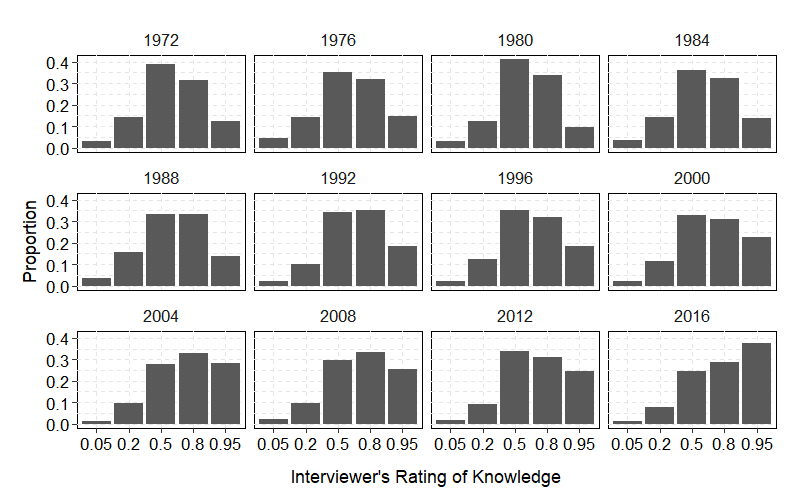
\includegraphics[width=\linewidth]{../outputs/anes_sbjkndist.png}
\end{figure}

\par \autoref{fig:anes_sbjkndist} shows the distribution of interviewer's rating of knowledge at each presidential election year of ANES time-series studies. The distribution is approximately normal for most of the early years, but the average level of knowledge is gradually over the years. In 2016, the distribution had the mode at 0.95. As a result, the knowledge distribution in 2008 and 2016 are similar to that of CCES knowledge score.    

\par Other variables are constructed from the following questions in ANES dataset:

\begin{itemize}
    \item Presidential vote choice (\texttt{vcf0704}). 1 is voting for Republican, 0 is voting for Democrat. All other responses are dropped from the analysis.
    \item Republican advantage in squared ideological distance. Constructed from respondent's self ideology location (\texttt{vcf0803}, \texttt{V720652} from 1972 data, \texttt{V763286} from 1976 data, \texttt{V800267} from 1980 data, \texttt{V840370} from 1984 data, \texttt{v000440} from 2000 data, and \texttt{v162171} and \texttt{v162171a} from 2016 data), Republican candidate's perceived ideological location (\texttt{vcf9096}), and Democratic candidate's perceived ideological location (\texttt{vcf9088}). Each ideological position variable is rescaled in -3 to 3 range (higher score indicates more Conservative). The final variable is scaled from -36 to 36 (higher score indicates that perceived ideological position of Republican candidate is closer than the perceived ideological position of Democratic candidate to self ideology position).
    \item The retrospective evaluation of national economy (\texttt{vcf0870}, \texttt{vcf0871}, \texttt{v720780} from 1972 data, and \texttt{v763139} from 1976 data). The variable is scaled from gotten much worse (-2) to gotten much better (2). The scale in election years with Democratic party as incumbent is reverse scaled so higher score advantages Republican candidate. 
    \item Party identity (\texttt{vcf0301}). Scaled from strong Democrat (-2) to strong Republican (2).
    \item Gender (\texttt{vcf0104}). 1 is female and 0 is male.
    \item Age (\texttt{vcf0101}).
    \item Race (\texttt{vcf0106}). Dummy variable is created for ethnic minority (i.e., non-White) respondents.
    \item Family income (\texttt{v720420} from 1972 data, \texttt{v763507} from 1976 data, \texttt{v800686} from 1980 data, \texttt{v840680} from 1984 data, \texttt{v880520} from 1988 data, \texttt{v924104} from 1992 data, \texttt{v960701} from 1996 data, \texttt{v000994} from 2000 data, \texttt{v04329x} from 2004 data, \texttt{v083248x} from 2008 data, \texttt{incgroup\_prepost\_x} from 2012 data, and \texttt{v161361x} and \texttt{v162309x} from 2016 data). Rescaled as a percentile.
    \item Education (\texttt{v720300} from 1972 data, \texttt{v763389} from 1976 data, \texttt{v800436} from 1980 data, \texttt{v840438} from 1984 data, \texttt{v880422} from 1988 data, \texttt{v923905} and \texttt{923908} from 1992 data, \texttt{v960607} and \texttt{960610} from 1996 data, \texttt{v000913} from 2000 data, \texttt{v043254} from 2004 data, \texttt{v083218x} from 2008 data, \texttt{dem\_edu} from 2012 data, and \texttt{vV161270} from 2016 data). Converted to the scale from 0 to 17.
    \item Religion (\texttt{vcf0128}, \texttt{v161247a} and \texttt{v161247b} from 2016 data). Creating dummy variables for Protestant and Catholic.
\end{itemize}

\subsection{Results for Demographic Controls} 

\par Following figures show the conditional coefficients of demographic control variables on the presidential vote choice (i.e., 1 = vote Republican, 0 = vote Democratic) in each presidential election year. Coefficients for individual preference variables are included in the main text. 

\begin{figure}[ht!!!]
    \caption{The impact of demographic variables on presidential Vote Choice (1 = Republican, 0 = Democrat) in ANES Part I (1972-2016)}
    \label{fig:anescoefplot_dem1}
    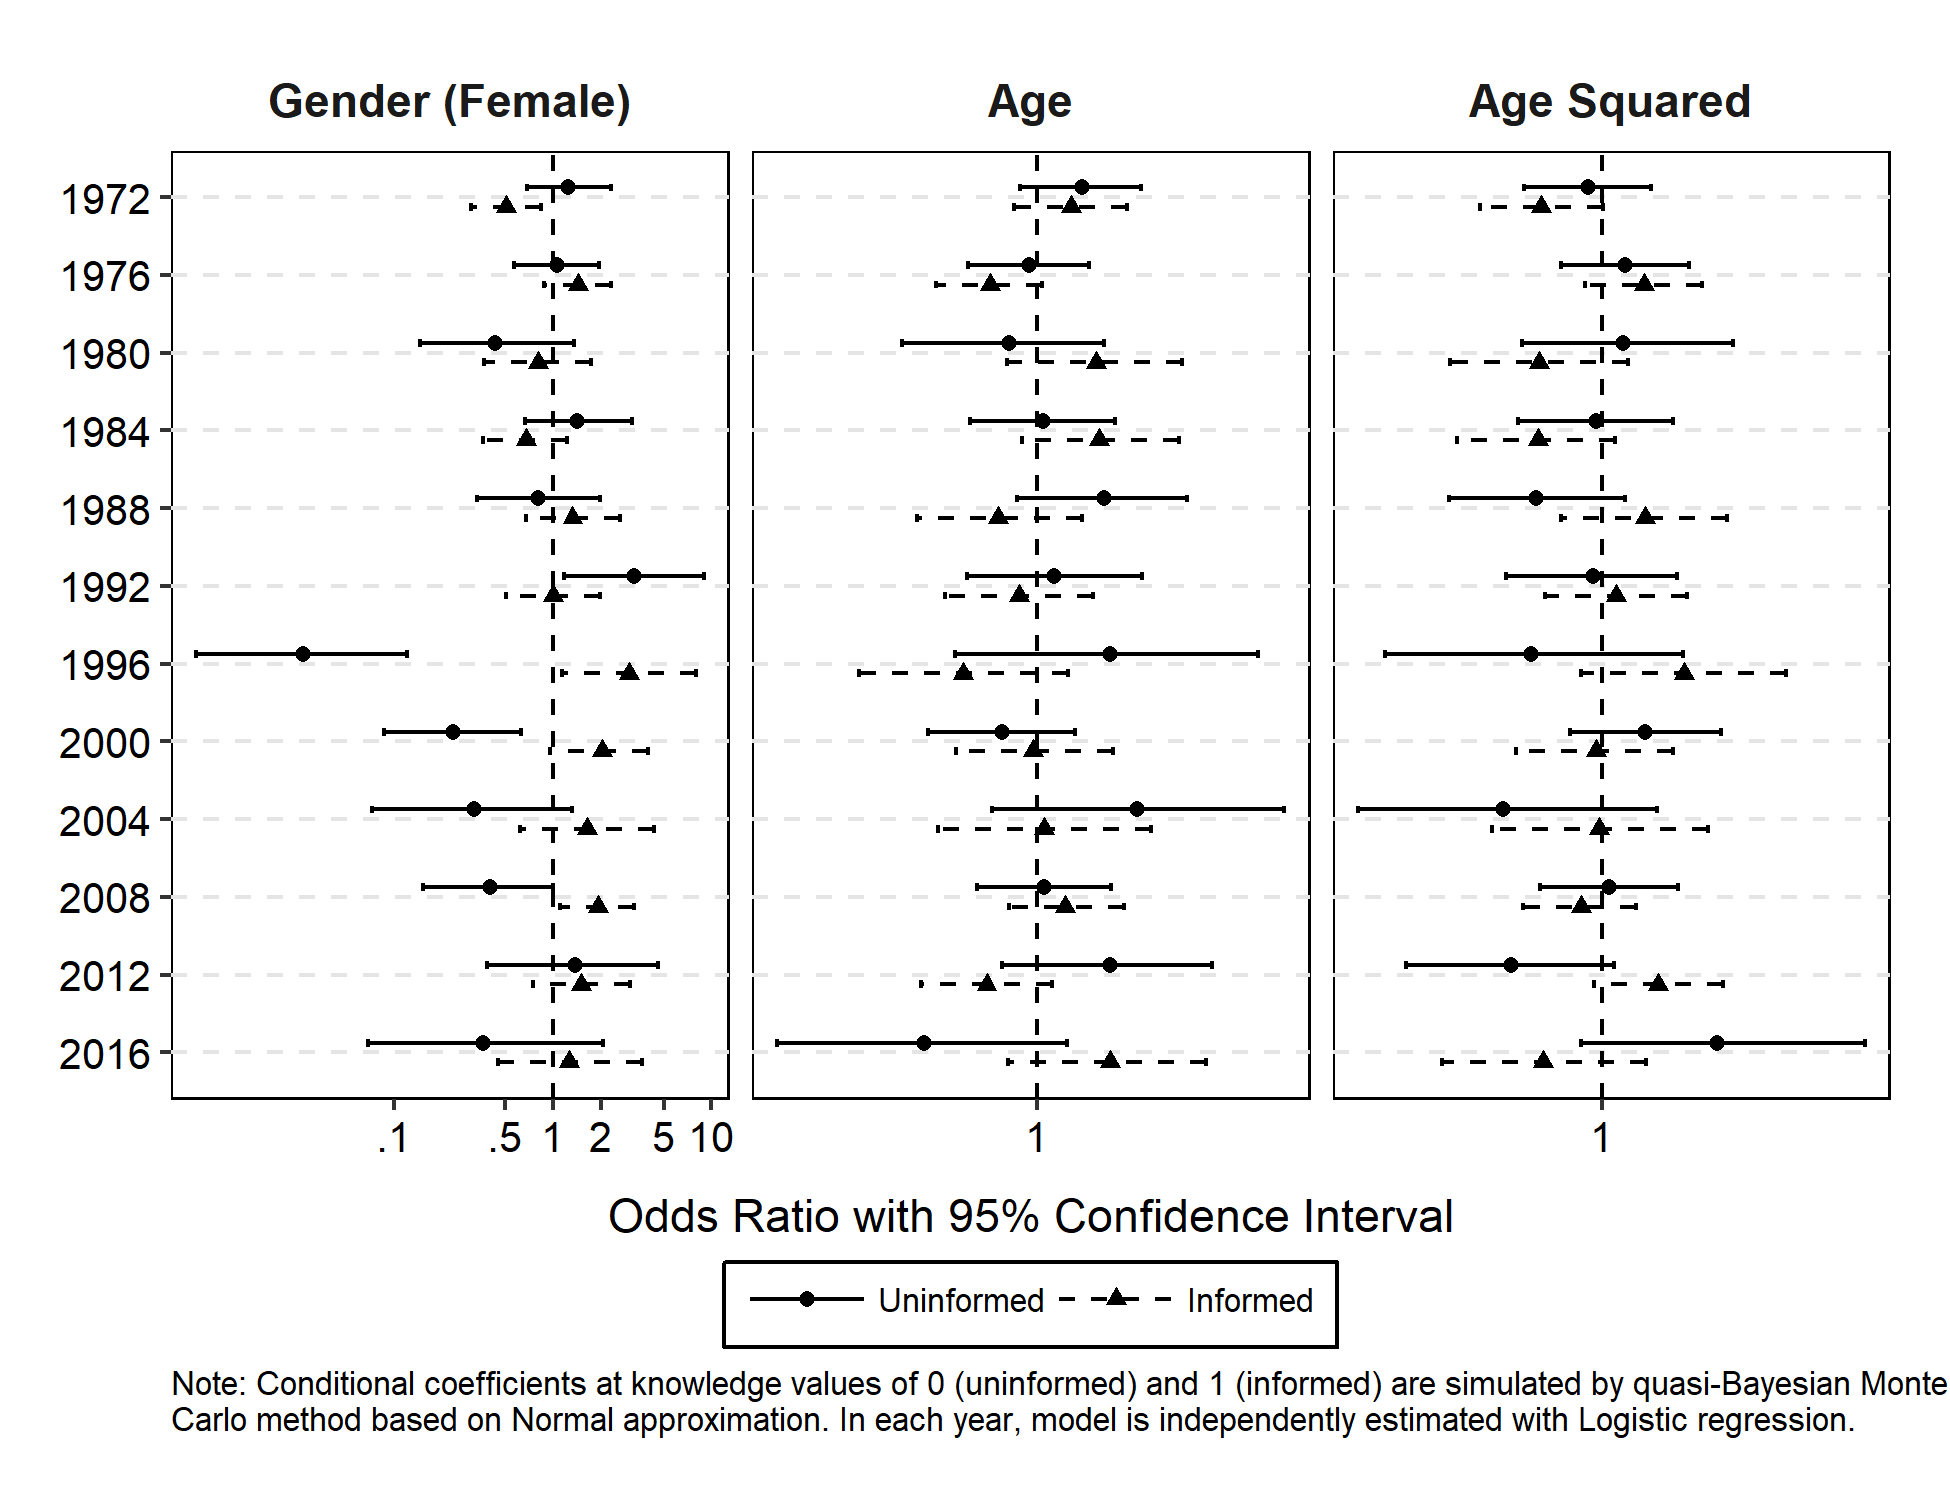
\includegraphics[width=\linewidth]{../outputs/m1sq_anescoefplot_dem1.png}
\end{figure}

\begin{figure}[ht!!!]
    \caption{The impact of demographic variables on presidential Vote Choice (1 = Republican, 0 = Democrat) in ANES Part II (1972-2016)}
    \label{fig:anescoefplot_dem2}
    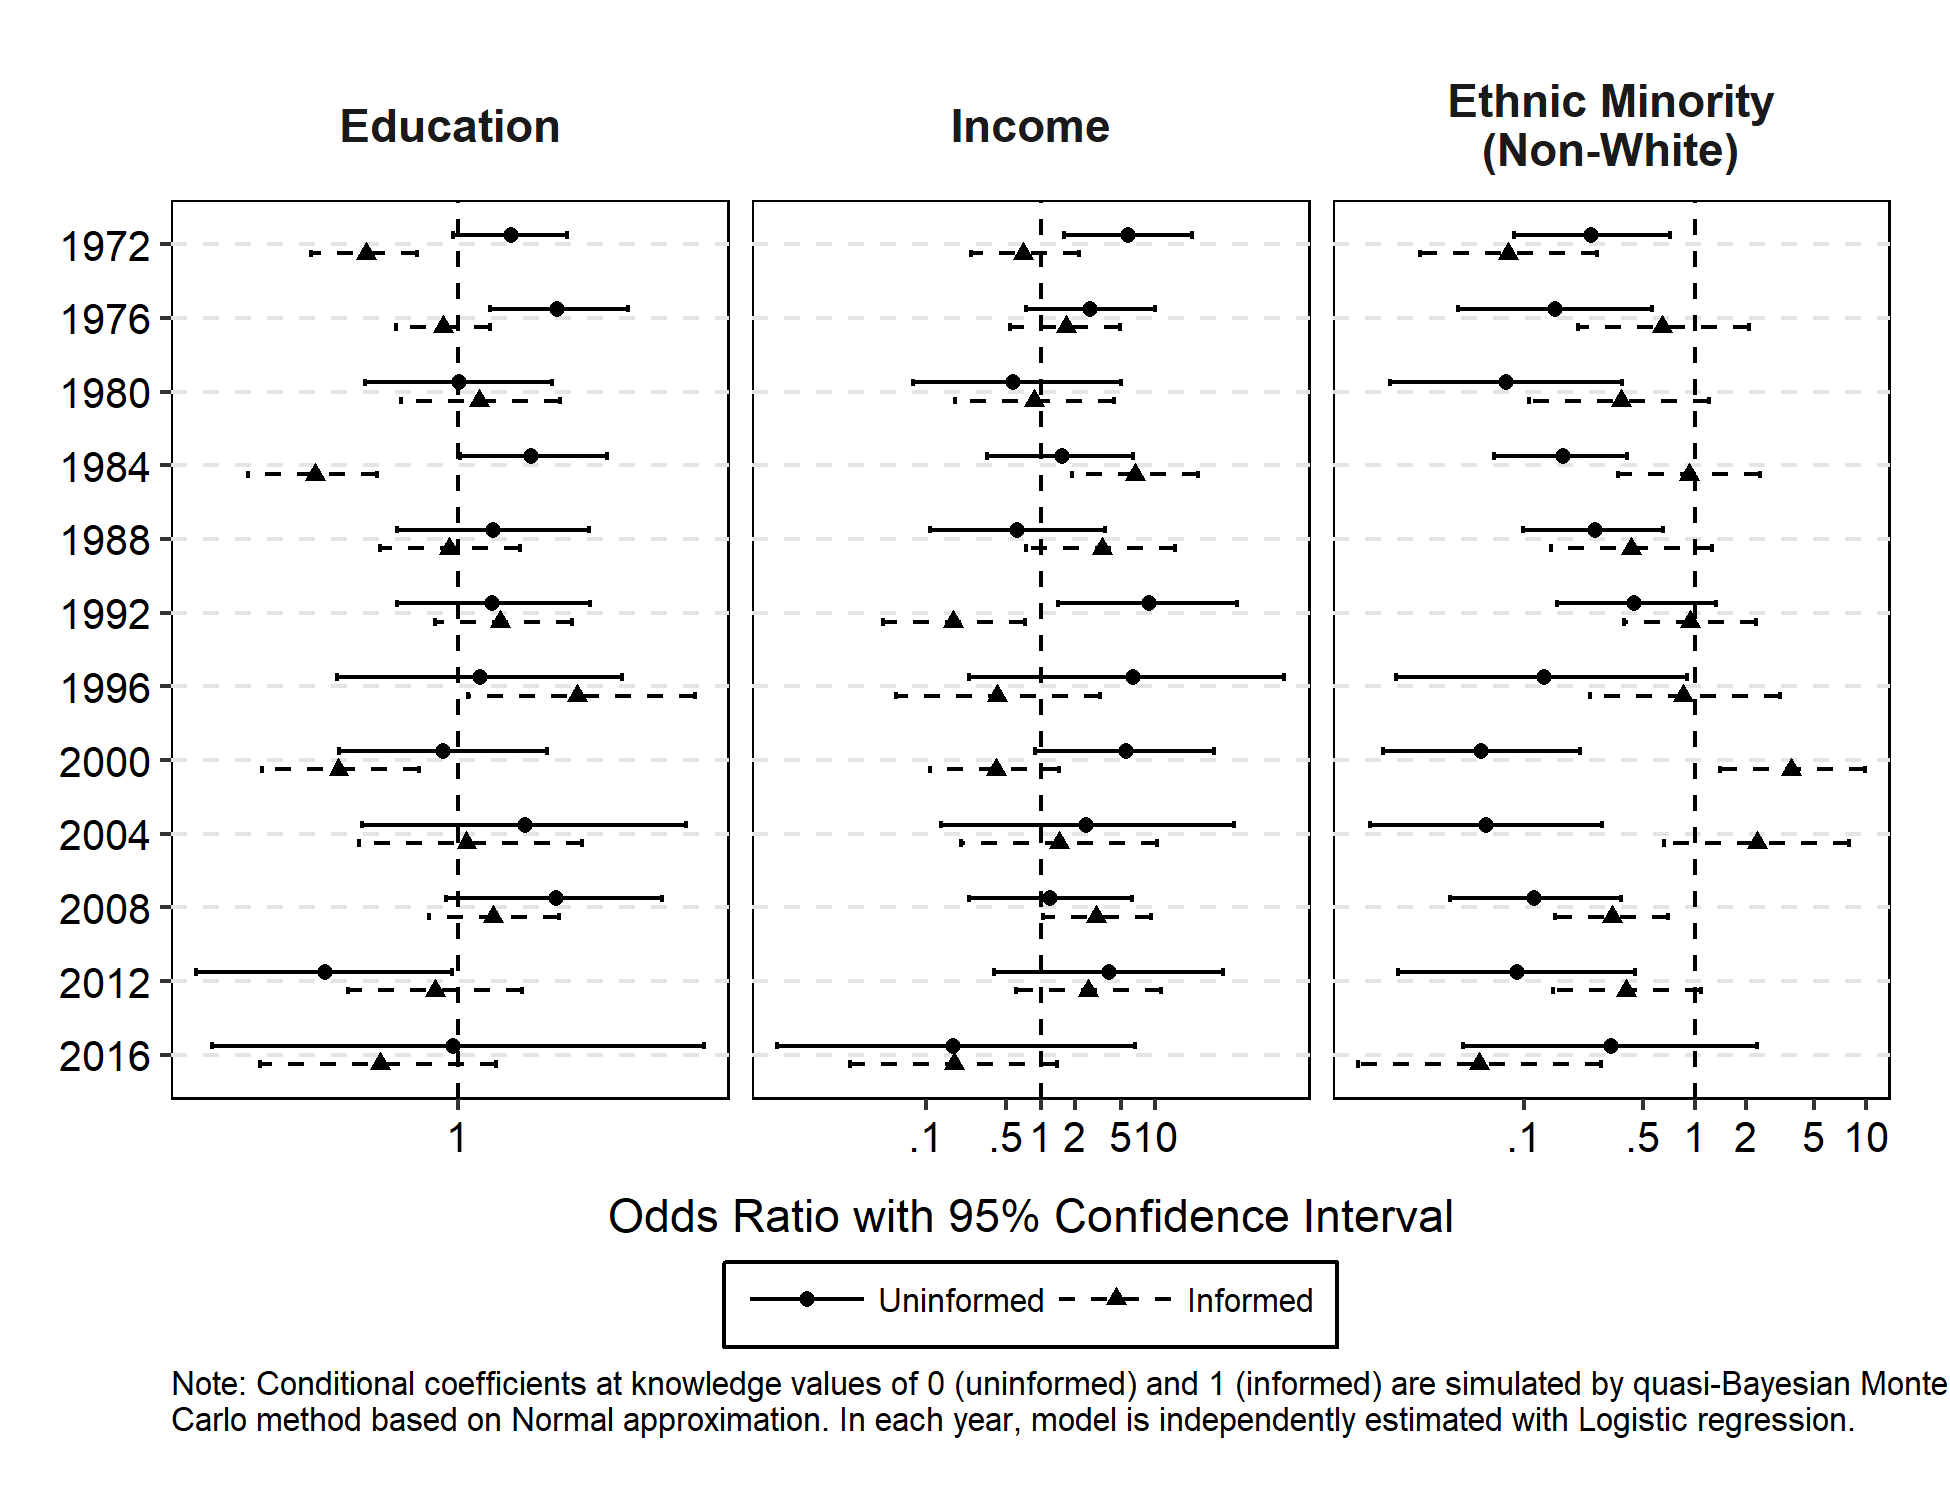
\includegraphics[width=\linewidth]{../outputs/m1sq_anescoefplot_dem2.png}
\end{figure}

\begin{figure}[ht!!!]
    \caption{The impact of demographic variables on presidential Vote Choice (1 = Republican, 0 = Democrat) in ANES Part III (1972-2016)}
    \label{fig:anescoefplot_dem3}
    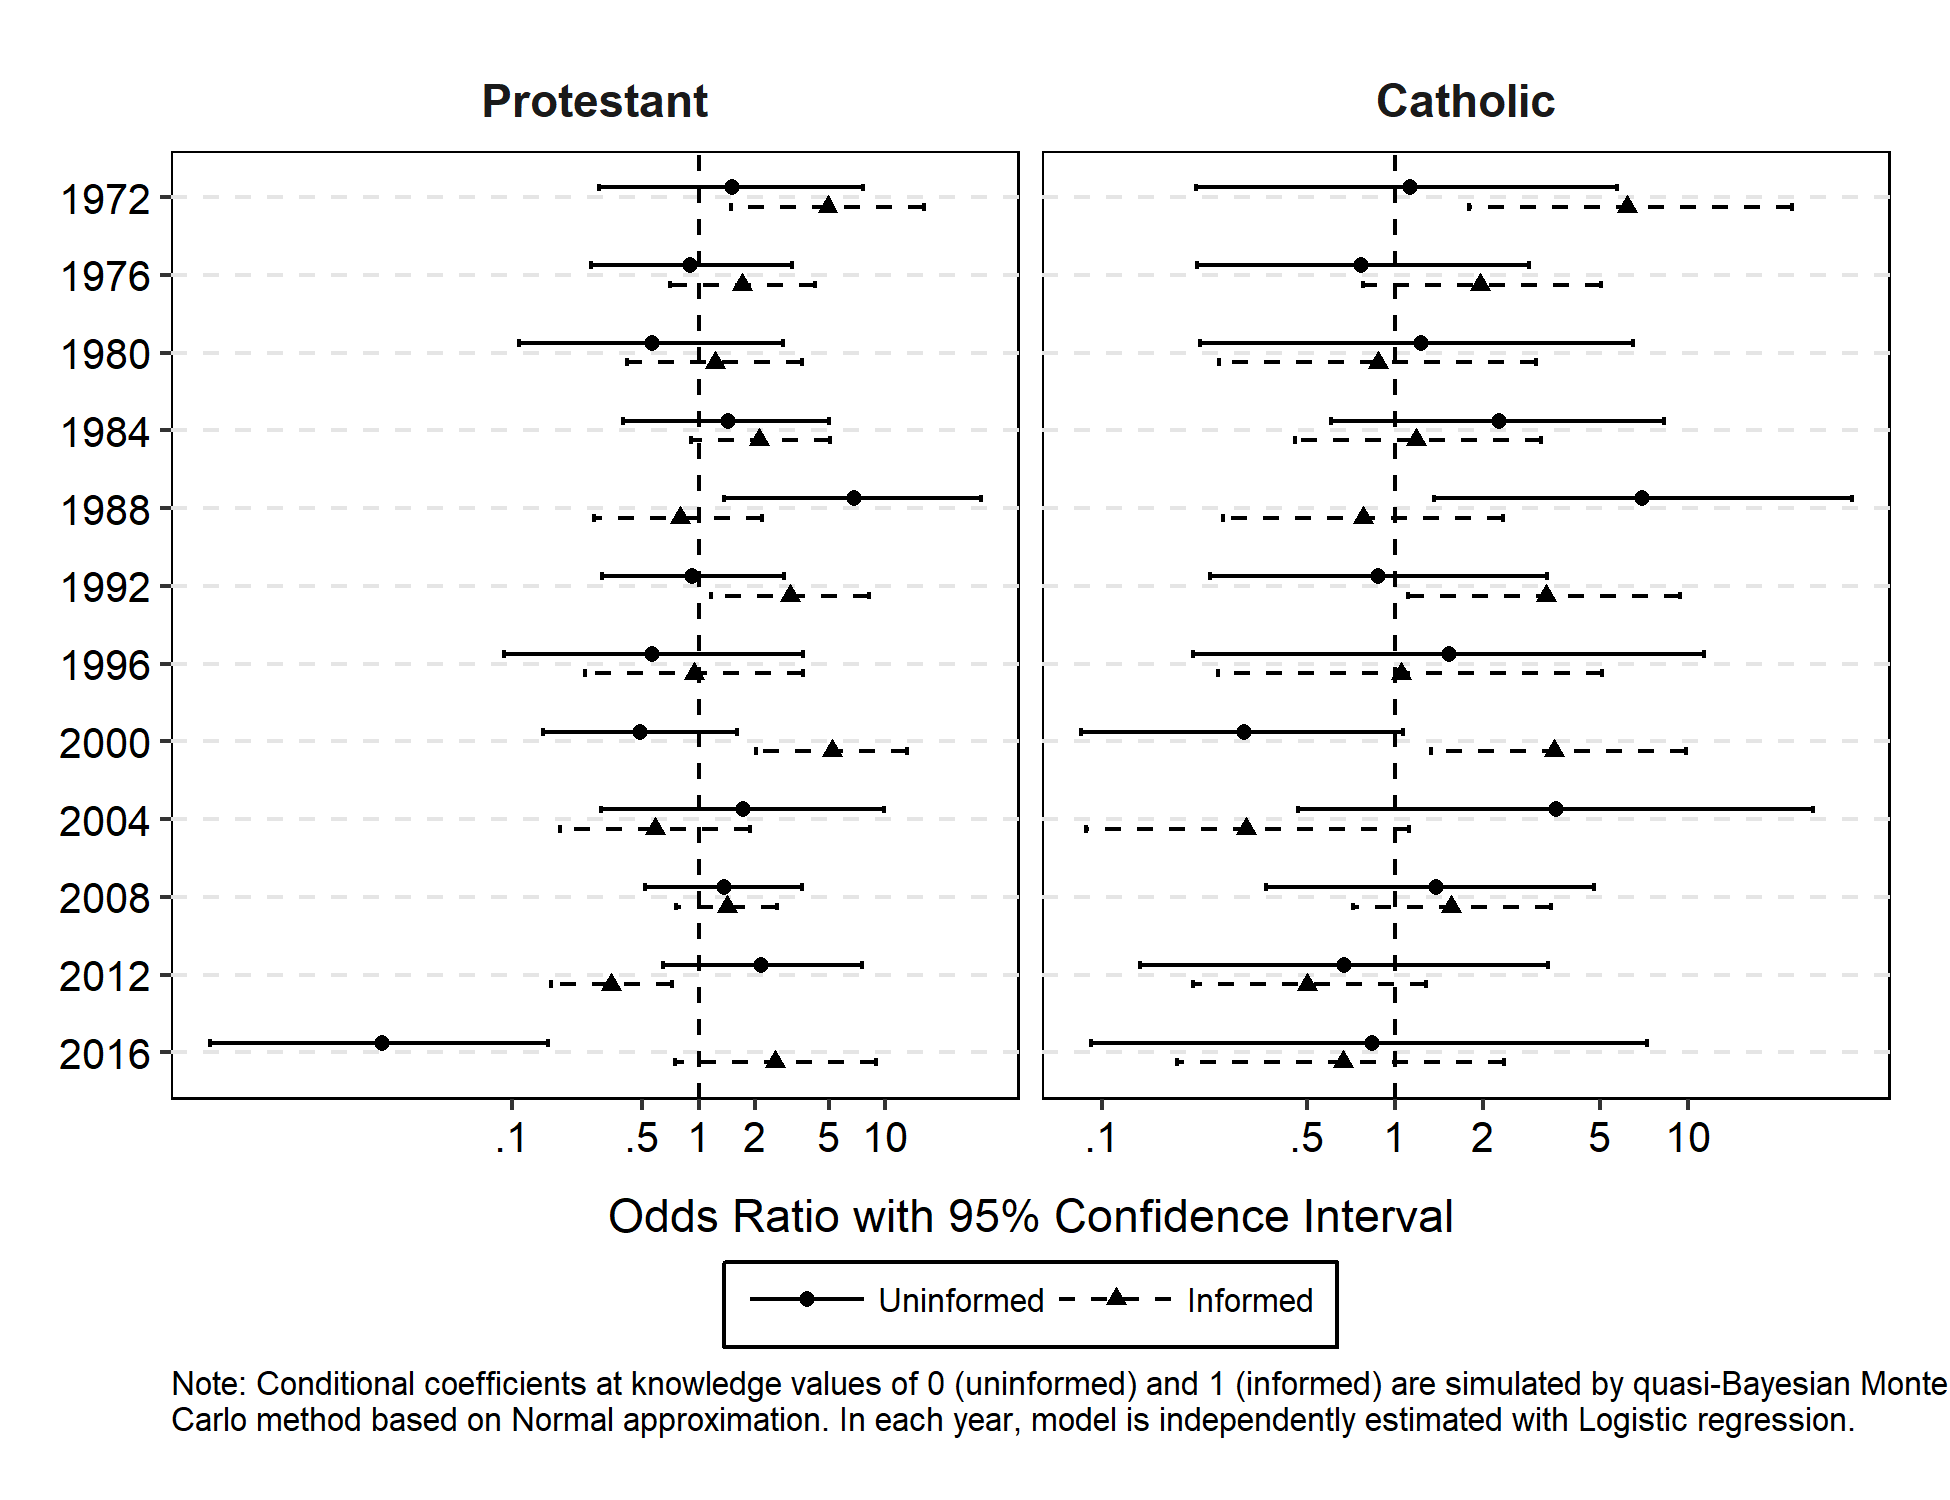
\includegraphics[width=\linewidth]{../outputs/m1sq_anescoefplot_dem3.png}
\end{figure}

\clearpage
\subsection{EDV Models Using Predictions Based on Voter Profiles from Different Years}

\begin{figure}[ht!!!]
    \caption{National partisan environment and incumbent party explain predicted probability of Republican vote in ANES (1972-2016), estimated with voter profiles from different years}
    \label{fig:anespredtable}
    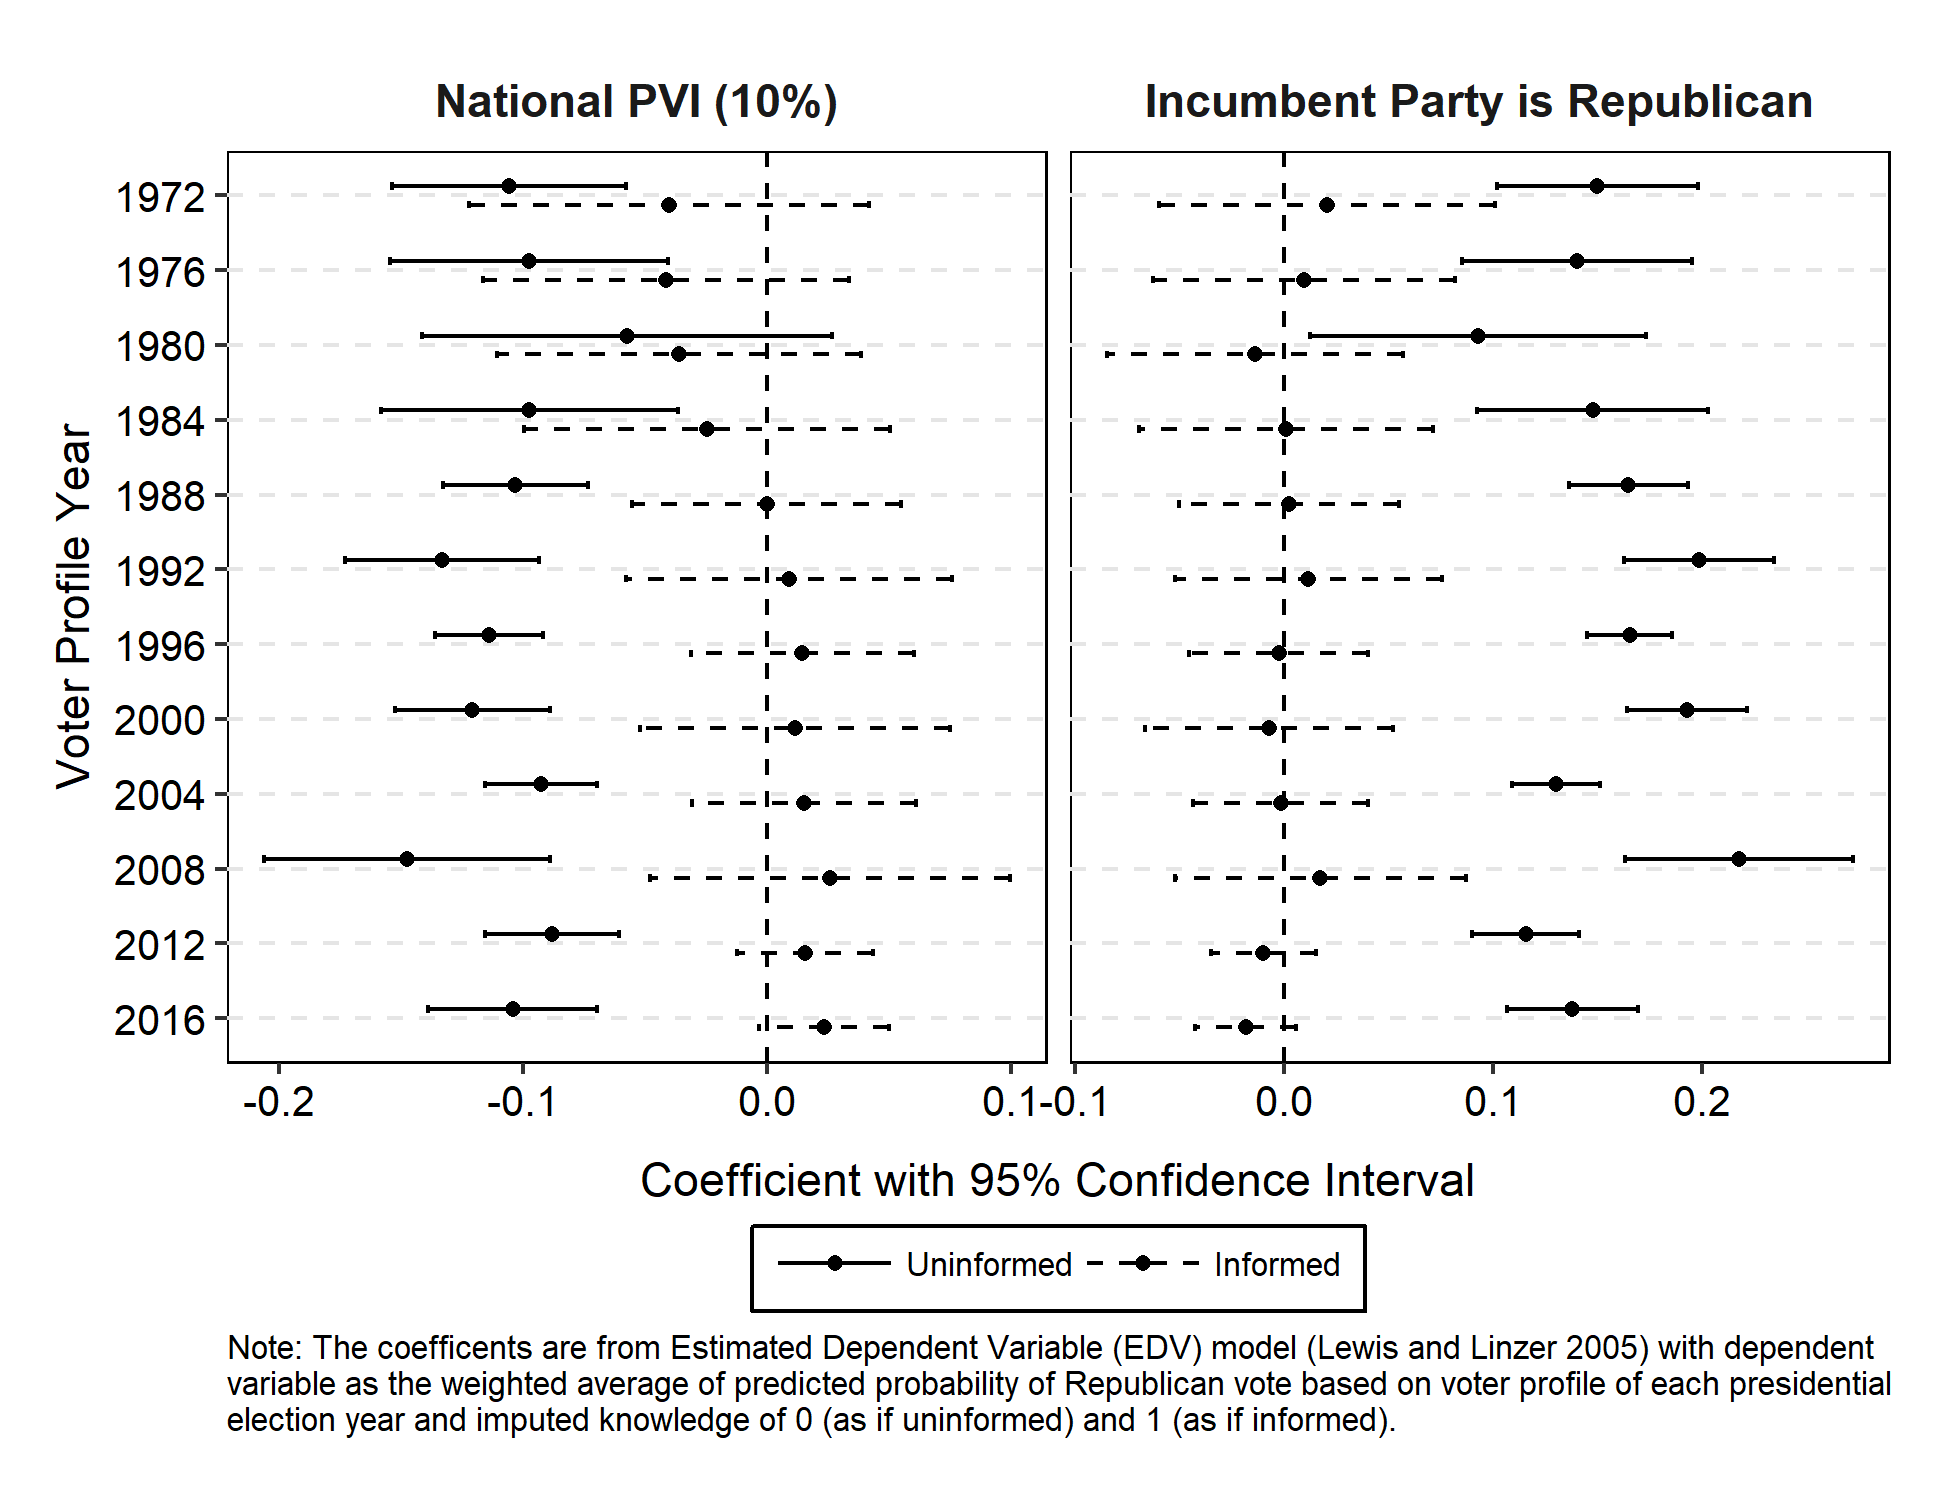
\includegraphics[width=\linewidth]{../outputs/m1sq_anespredtable.png}
\end{figure}

\par \autoref{fig:anespredtable} shows the coefficient from EDV regressions with national PVI and incumbent party (i.e., Republican = 1, Democrat = 0) as predictors. The outcome is the weighted average of the probability of Republican vote based on the voter profile from the given year and manipulated value of knowledge (i.e., either 0 = uninformed or 1 = informed). The result confirms that national PVI has a negative influence on the predicted Republican vote probability of uninformed voters with the voter profile from any given year (the coefficient is statistically significant at 5\% level for all but 1980 profile). Similarly, Republican being incumbent party has a consistently positive impact on the Republican vote probability of uninformed voters. On the other hand, two variables are never significant predictors of Republican voter probability of informed voters.        

\clearpage
\subsection{Analysis with Objective Knowledge}

\par The objective knowledge score from ANES is constructed from aggregating correct answers to following questions offered in each election year. 

\begin{itemize}
    \item 1972: \texttt{v720943}, \texttt{v720944}, \texttt{v720945}, \texttt{v720946a}, \texttt{v720947a}, \texttt{v720946b}, \texttt{v720947b}, \texttt{v720948}, \texttt{v720949}, \texttt{v720950}, and \texttt{v720951}  (\texttt{v720006} to code correct answer)
    \item 1976: \texttt{v763683} and \texttt{v763684}
    \item 1980: \texttt{v801028}, \texttt{v801029}, \texttt{v800826}, \texttt{v800829}, \texttt{v800913} (\texttt{v800823} is used to identify missing values, \texttt{vcf0977} and \texttt{vcf0978} from cumulative data are used to code correct answers)
    \item 1984: \texttt{v841006}, \texttt{v841007}, \texttt{v840741}, \texttt{v840745}, and \texttt{v840741} (\texttt{v840737} is used to identify missing values, \texttt{vcf0977} and \texttt{vcf0978} from cumulative data are used to code correct answers)
    \item 1988: \texttt{v880878}, \texttt{v880569}, \texttt{v880573}, \texttt{v880879}, \texttt{v880709}, \texttt{v880712}, \texttt{v880871}, \texttt{v880872}, \texttt{v880873}, \texttt{v880874}, \texttt{v880875}, \texttt{v880876}, and \texttt{v880877} (\texttt{v880565} is used to identify missing values, \texttt{vcf0977} and \texttt{vcf0978} from cumulative data are used to code correct answers)
    \item 1992: \texttt{v925951}, \texttt{v925113}, \texttt{v925117}, \texttt{v925952}, \texttt{v925435},\texttt{v925438}, \texttt{v925916}, \texttt{v925917}, \texttt{v925918}, \texttt{v925919}, \texttt{v925920}, and \texttt{v925921} (\texttt{v925109} is used to identify missing values, \texttt{vcf0977} and \texttt{vcf0978} from cumulative data are used to code correct answers)
    \item 1996: \texttt{v961072}, \texttt{v961010}, \texttt{v961014}, \texttt{v961073}, \texttt{v961068}, \texttt{v961070}, \texttt{v961189}, \texttt{v961190}, \texttt{v961191}, and \texttt{v961192} (\texttt{v961006} is used to identify missing values, \texttt{vcf0977} and \texttt{vcf0978} from cumulative data are used to code correct answers)
    \item 2000: \texttt{v001356}, \texttt{v001210}, \texttt{v001214}, \texttt{v001357}, \texttt{v001353a}, \texttt{v001354}, \texttt{v001447}, \texttt{v001450}, \texttt{v001453}, and \texttt{v001456} (\texttt{v001206} is used to identify missing values, \texttt{vcf0977} and \texttt{vcf0978} from cumulative data are used to code correct answers)
    \item 2004: \texttt{v045089}, \texttt{v045090}, \texttt{v045162}, \texttt{v045163}, \texttt{v045164}, and \texttt{v045165}
    \item 2008: \texttt{v085066}, \texttt{v085067}, \texttt{v085120}, \texttt{v085120}, \texttt{v085121}, \texttt{v085122}, and \texttt{v085123} (\texttt{PELOSI\_Level1}, \texttt{CHENEY\_Level1}, \texttt{BROWN\_Level1}, and \texttt{ROBERTS\_Level1} in 2008 Office Recognition Coding Data are used to code correct answers)
    \item 2012: \texttt{preknow\_prestimes}, \texttt{preknow\_sizedef}, \texttt{preknow\_senterm}, \texttt{preknow\_medicare}, \texttt{preknow\_leastsp}, \texttt{knowl\_housemaj}, \texttt{knowl\_senmaj}, \texttt{ofcrec\_speaker\_correct}, \texttt{ofcrec\_vp\_correct}, \texttt{ofcrec\_pmuk\_correct}, and \texttt{ofcrec\_cj\_correct}
    \item 2016: \texttt{v161515}, \texttt{v161516}, \texttt{v162072}, \texttt{v162073a}, \texttt{v162074a}, \texttt{162075a}, \texttt{162076a}
\end{itemize}

\noindent To generate the comparable measure of objective knowledge, I train simple one-dimensional Item Response Theory (IRT) score within each survey year. The exported score has a mean of approximately 0 and the standard deviation of 1. I rescaled the score so that it has a mean of 0.5 and a standard deviation of 0.5. The conditional coefficients are calculated by setting this variable at 0 (uninformed, 2SD below the mean) and 1 (informed, 2SD above the mean). 

\begin{figure}[ht!!!]
    \caption{The distribution of objective knowledge score (1972-2016)}
    \label{fig:anes_objkndist}
    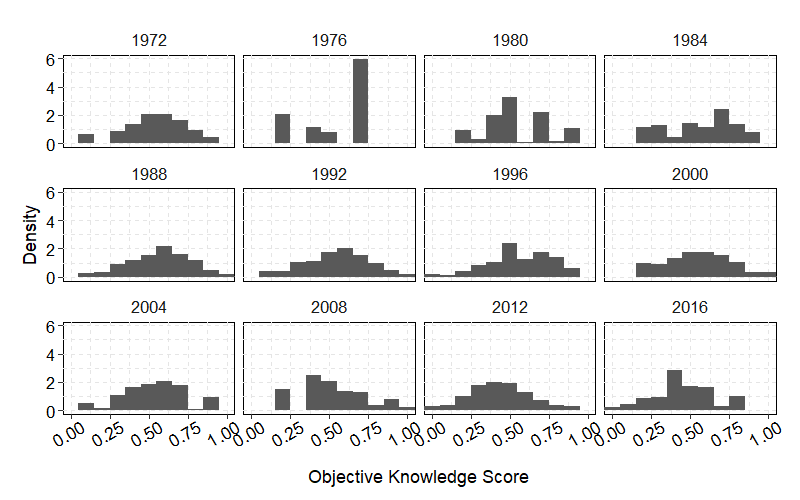
\includegraphics[width=\linewidth]{../outputs/anes_objkndist.png}
\end{figure}

\noindent \autoref{fig:anes_objkndist} shows the distribution of objective knowledge score at each given year. With the exception of 1976, the score in each year approximately looks normal. In 1976, only two factual test knowledge questions were offered, so the results should be interpreted with caution.

\par \autoref{fig:v2anescoefplot}, \autoref{fig:v2anescoefplot_dem1}, \autoref{fig:v2anescoefplot_dem2}, and \autoref{fig:v2anescoefplot_dem3} show the results of models predicting Republican vote with individual preference and demography variables. 

\begin{figure}[ht!!!]
    \caption{The impact of individual preference variables on presidential Vote Choice (1 = Republican, 0 = Democrat) in ANES (1972-2016) (objective knowledge)}
    \label{fig:v2anescoefplot}
    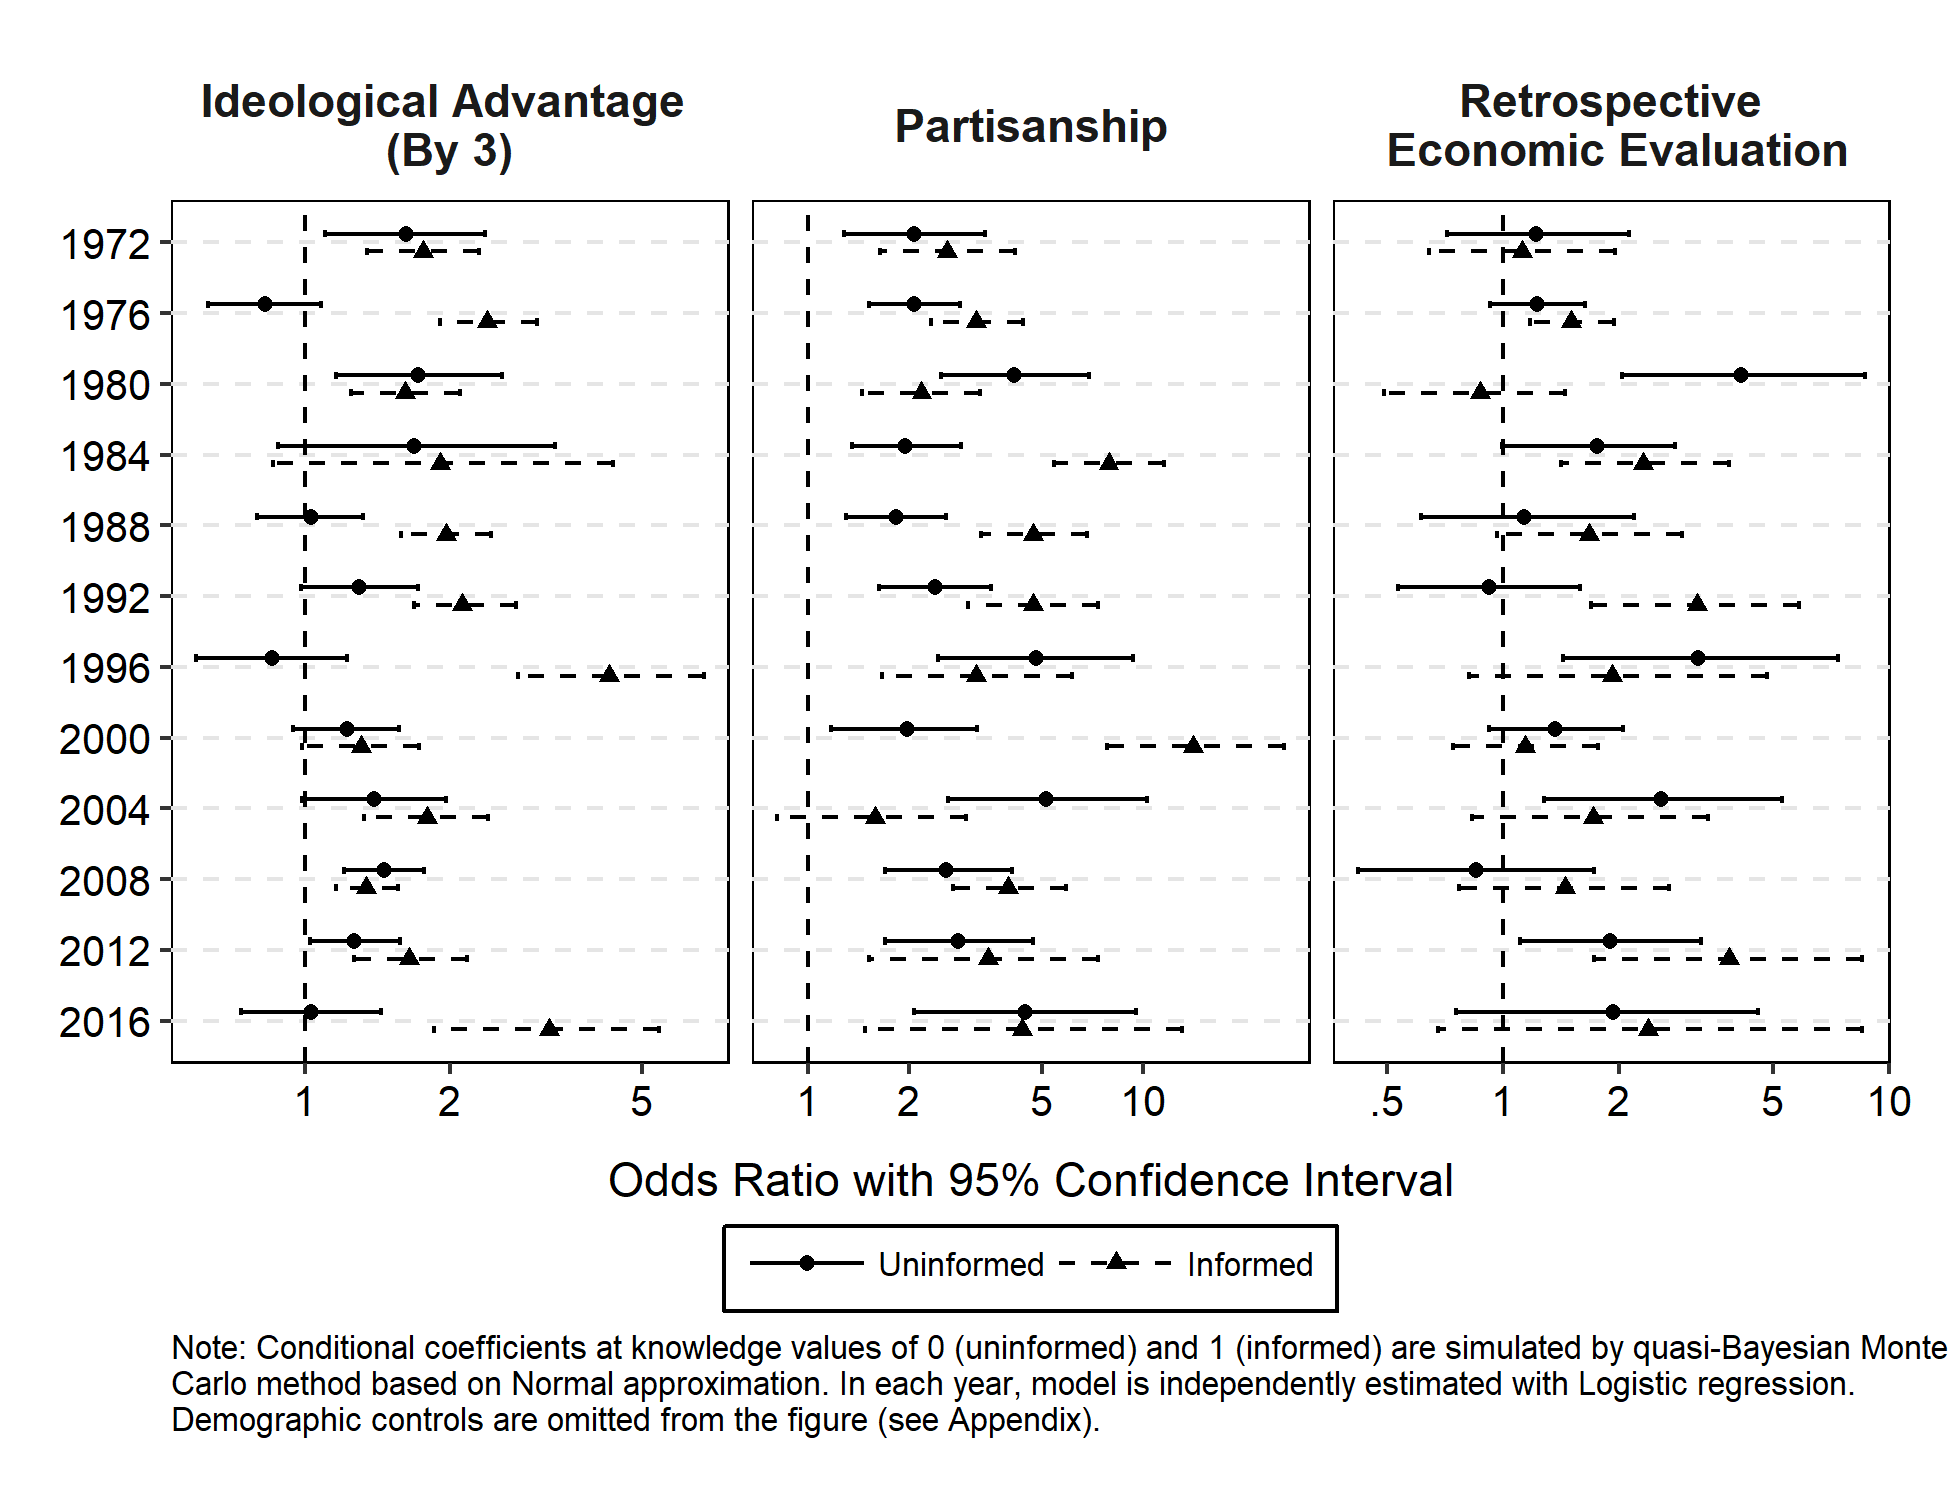
\includegraphics[width=\linewidth]{../outputs/m2sq_anescoefplot.png}
\end{figure}

\begin{figure}[ht!!!]
    \caption{The impact of demographic variables on presidential Vote Choice (1 = Republican, 0 = Democrat) in ANES Part I (1972-2016) (objective knowledge)}
    \label{fig:v2anescoefplot_dem1}
    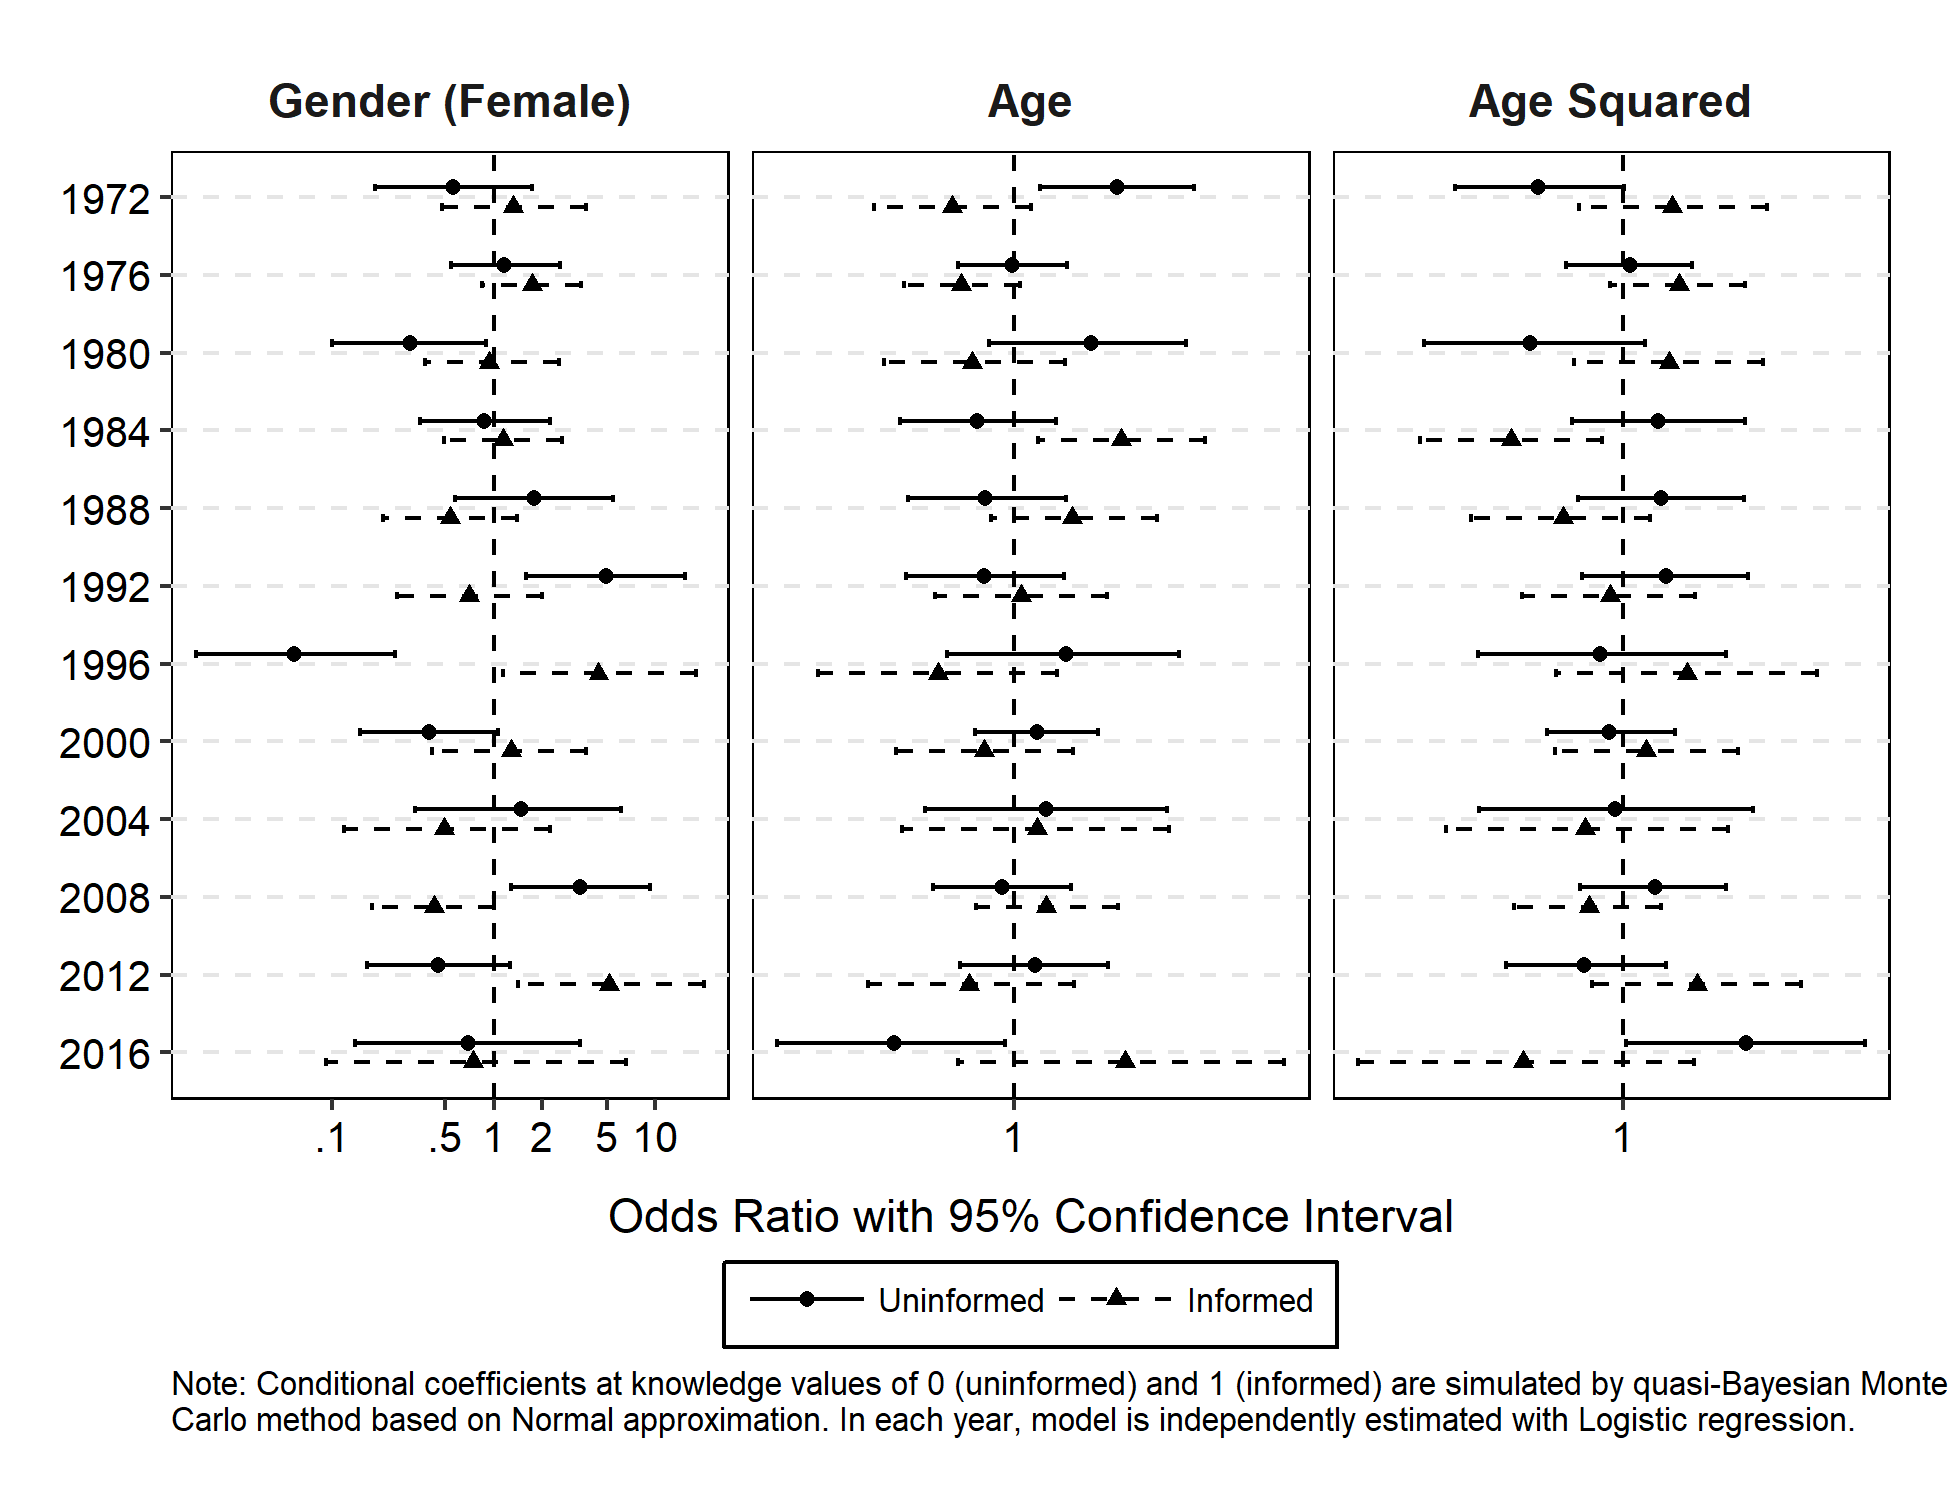
\includegraphics[width=\linewidth]{../outputs/m2sq_anescoefplot_dem1.png}
\end{figure}

\begin{figure}[ht!!!]
    \caption{The impact of demographic variables on presidential Vote Choice (1 = Republican, 0 = Democrat) in ANES Part II (1972-2016) (objective knowledge)}
    \label{fig:v2anescoefplot_dem2}
    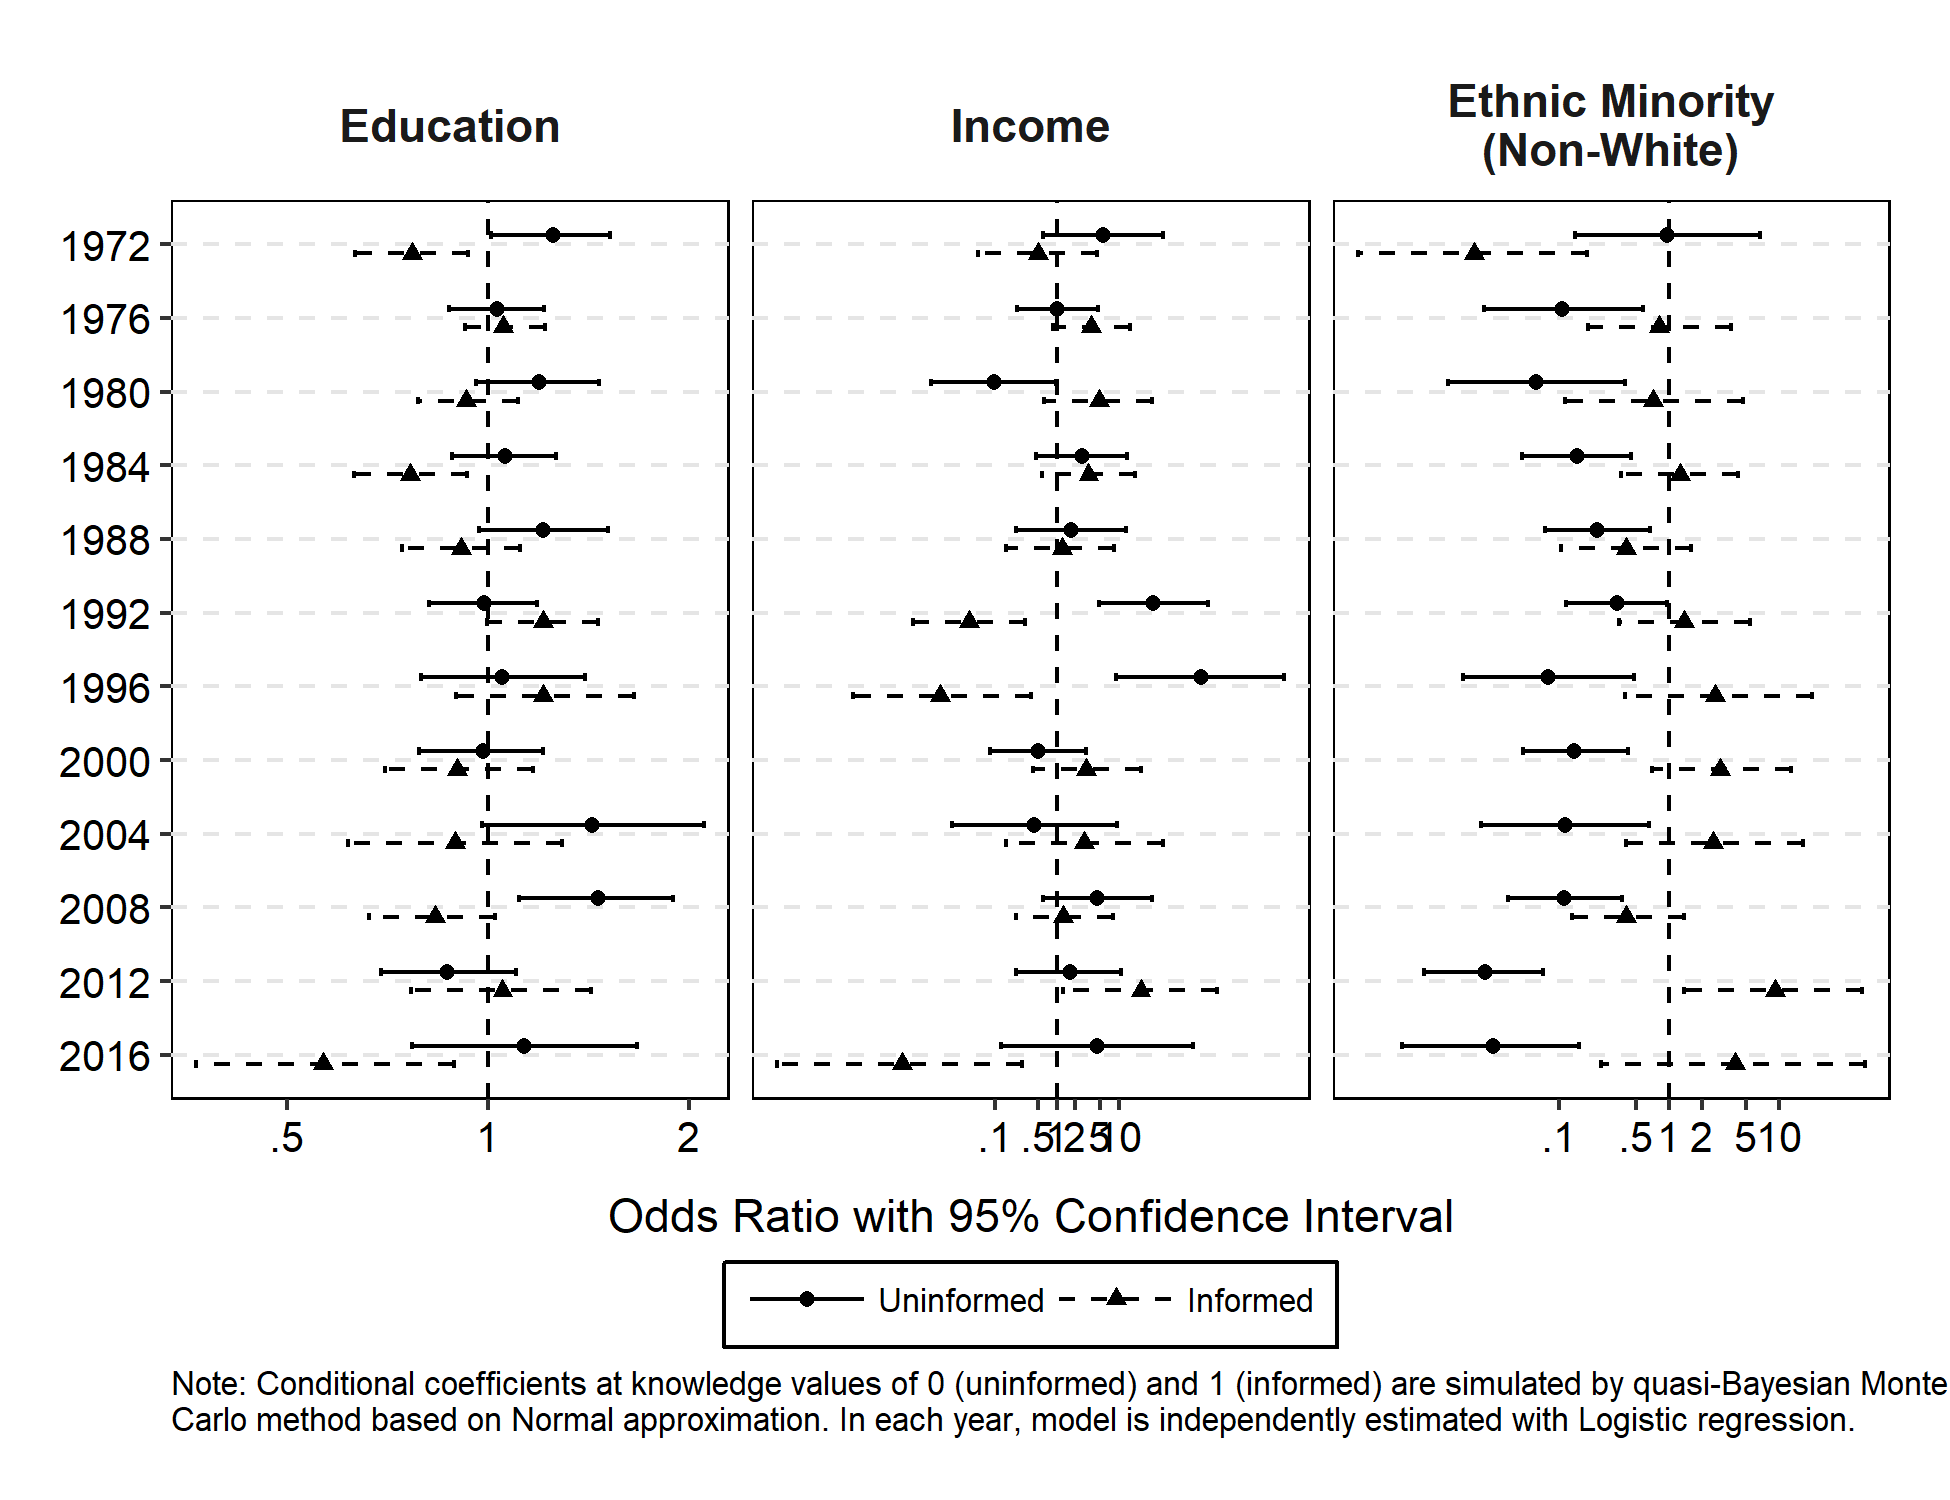
\includegraphics[width=\linewidth]{../outputs/m2sq_anescoefplot_dem2.png}
\end{figure}

\begin{figure}[ht!!!]
    \caption{The impact of demographic variables on presidential Vote Choice (1 = Republican, 0 = Democrat) in ANES Part III (1972-2016) (objective knowledge)}
    \label{fig:v2anescoefplot_dem3}
    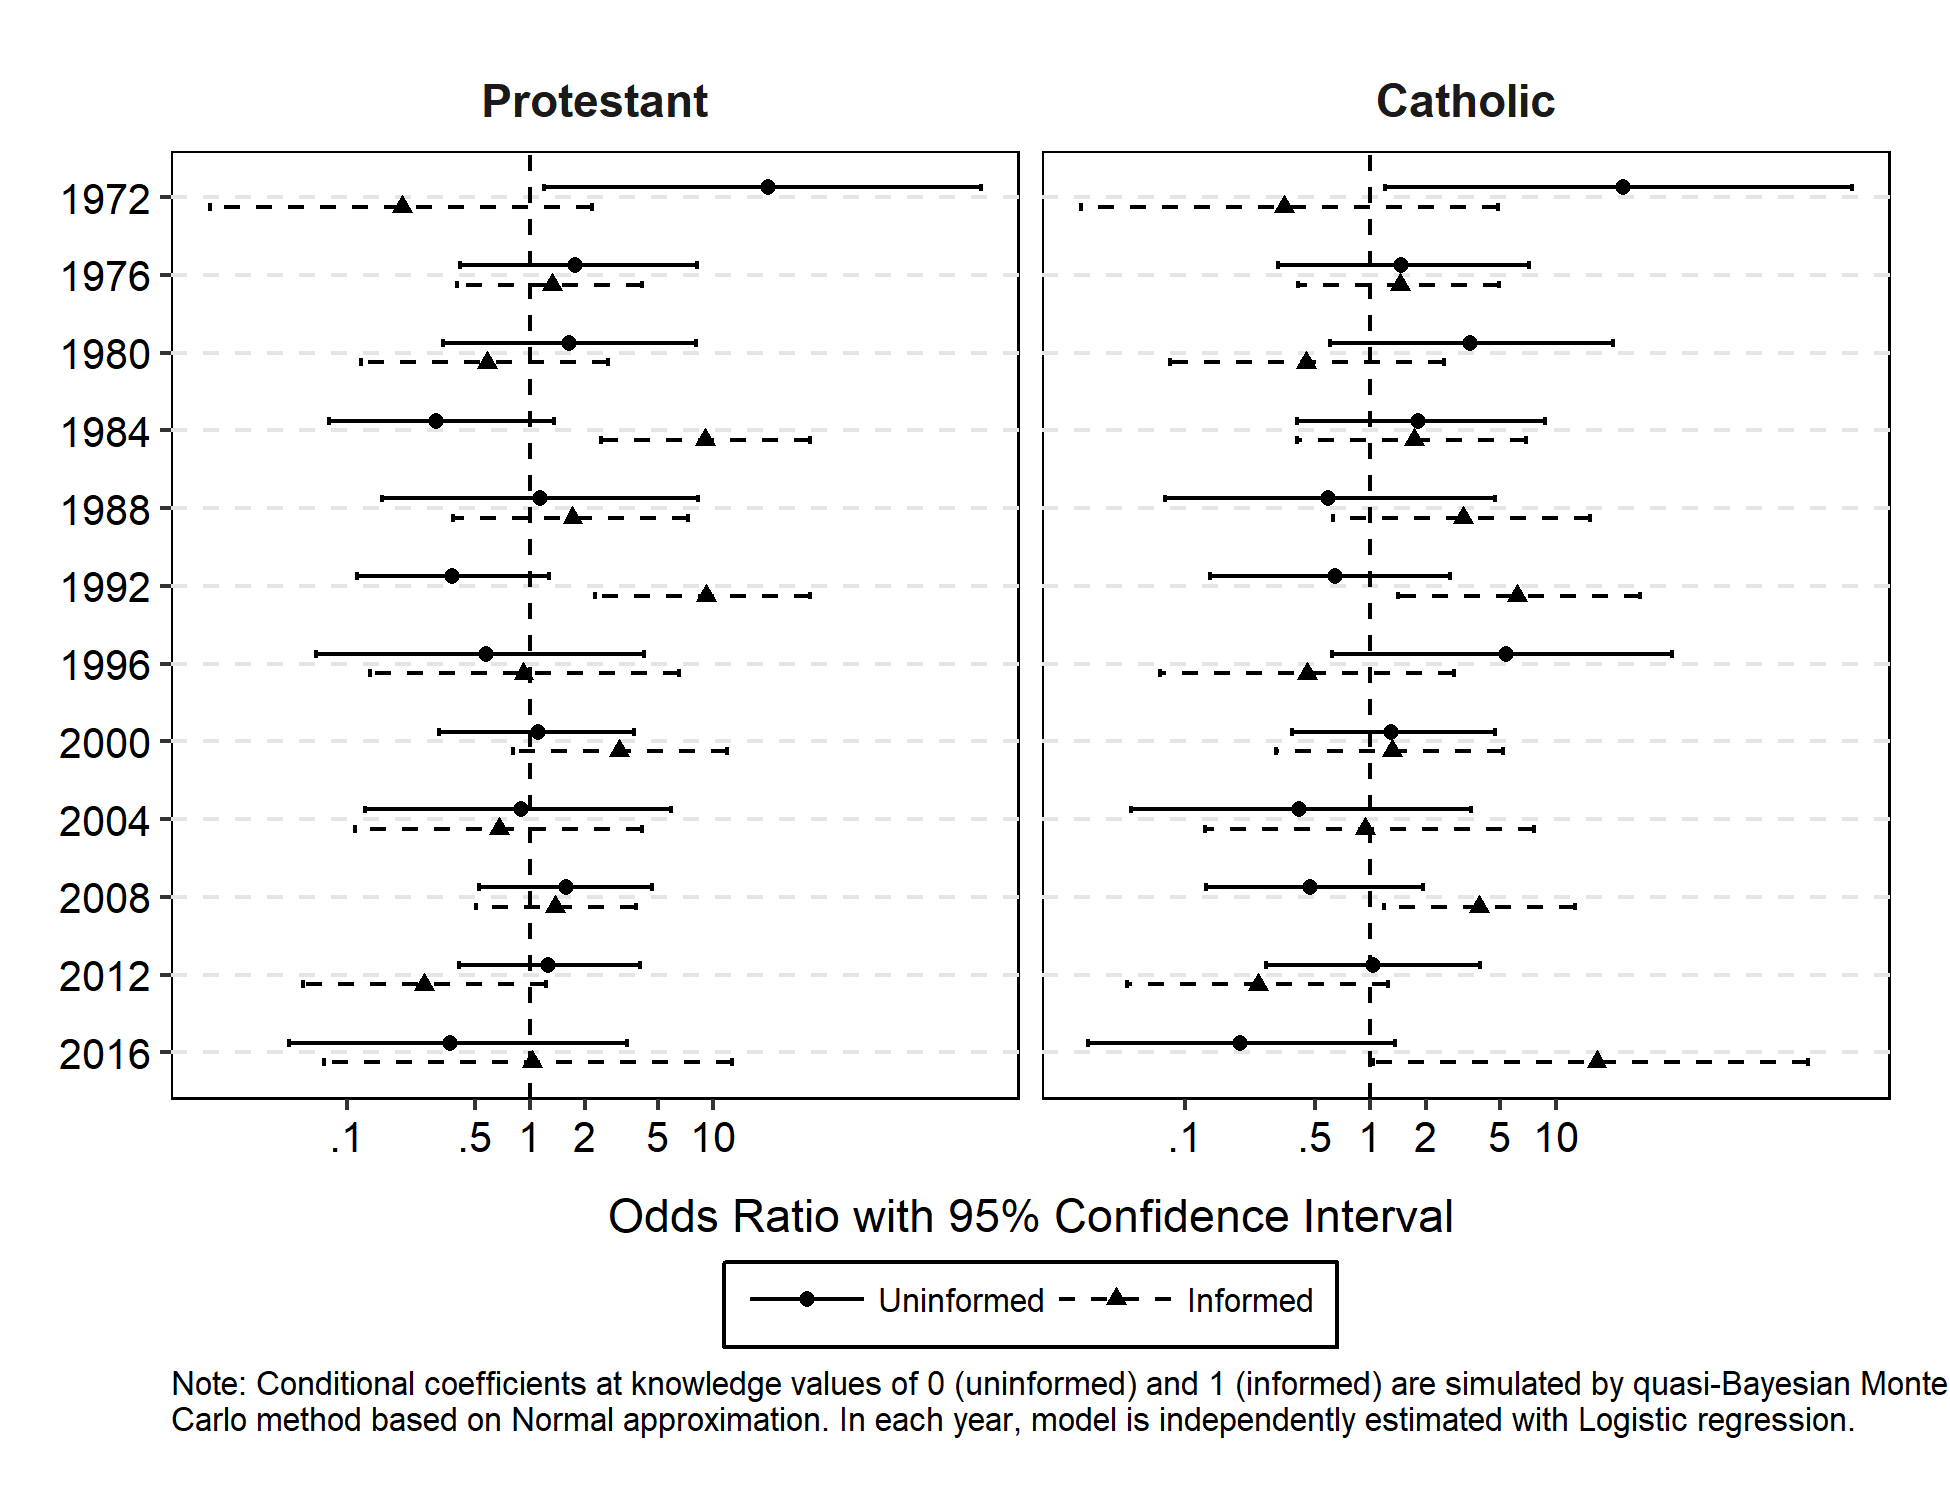
\includegraphics[width=\linewidth]{../outputs/m2sq_anescoefplot_dem3.png}
\end{figure}

\par In addition, \autoref{fig:v2anespredtable} shows the result comparable to \autoref{fig:anespredtable}, this time for objective knowledge. The result shows that the negative impact of national PVI on Republican vote choice persists (coefficient from EDV regression is statistically significant at 5\% level for all years but 2008). On the other hand, the effect of the incumbent party is weak and not statistically significant for most of the years.   

\begin{figure}[ht!!!]
    \caption{National partisan environment explains, but incumbent party does not explain predicted probability of Republican vote in ANES (1972-2016), estimated with voter profiles from different years (objective knowledge)}
    \label{fig:v2anespredtable}
    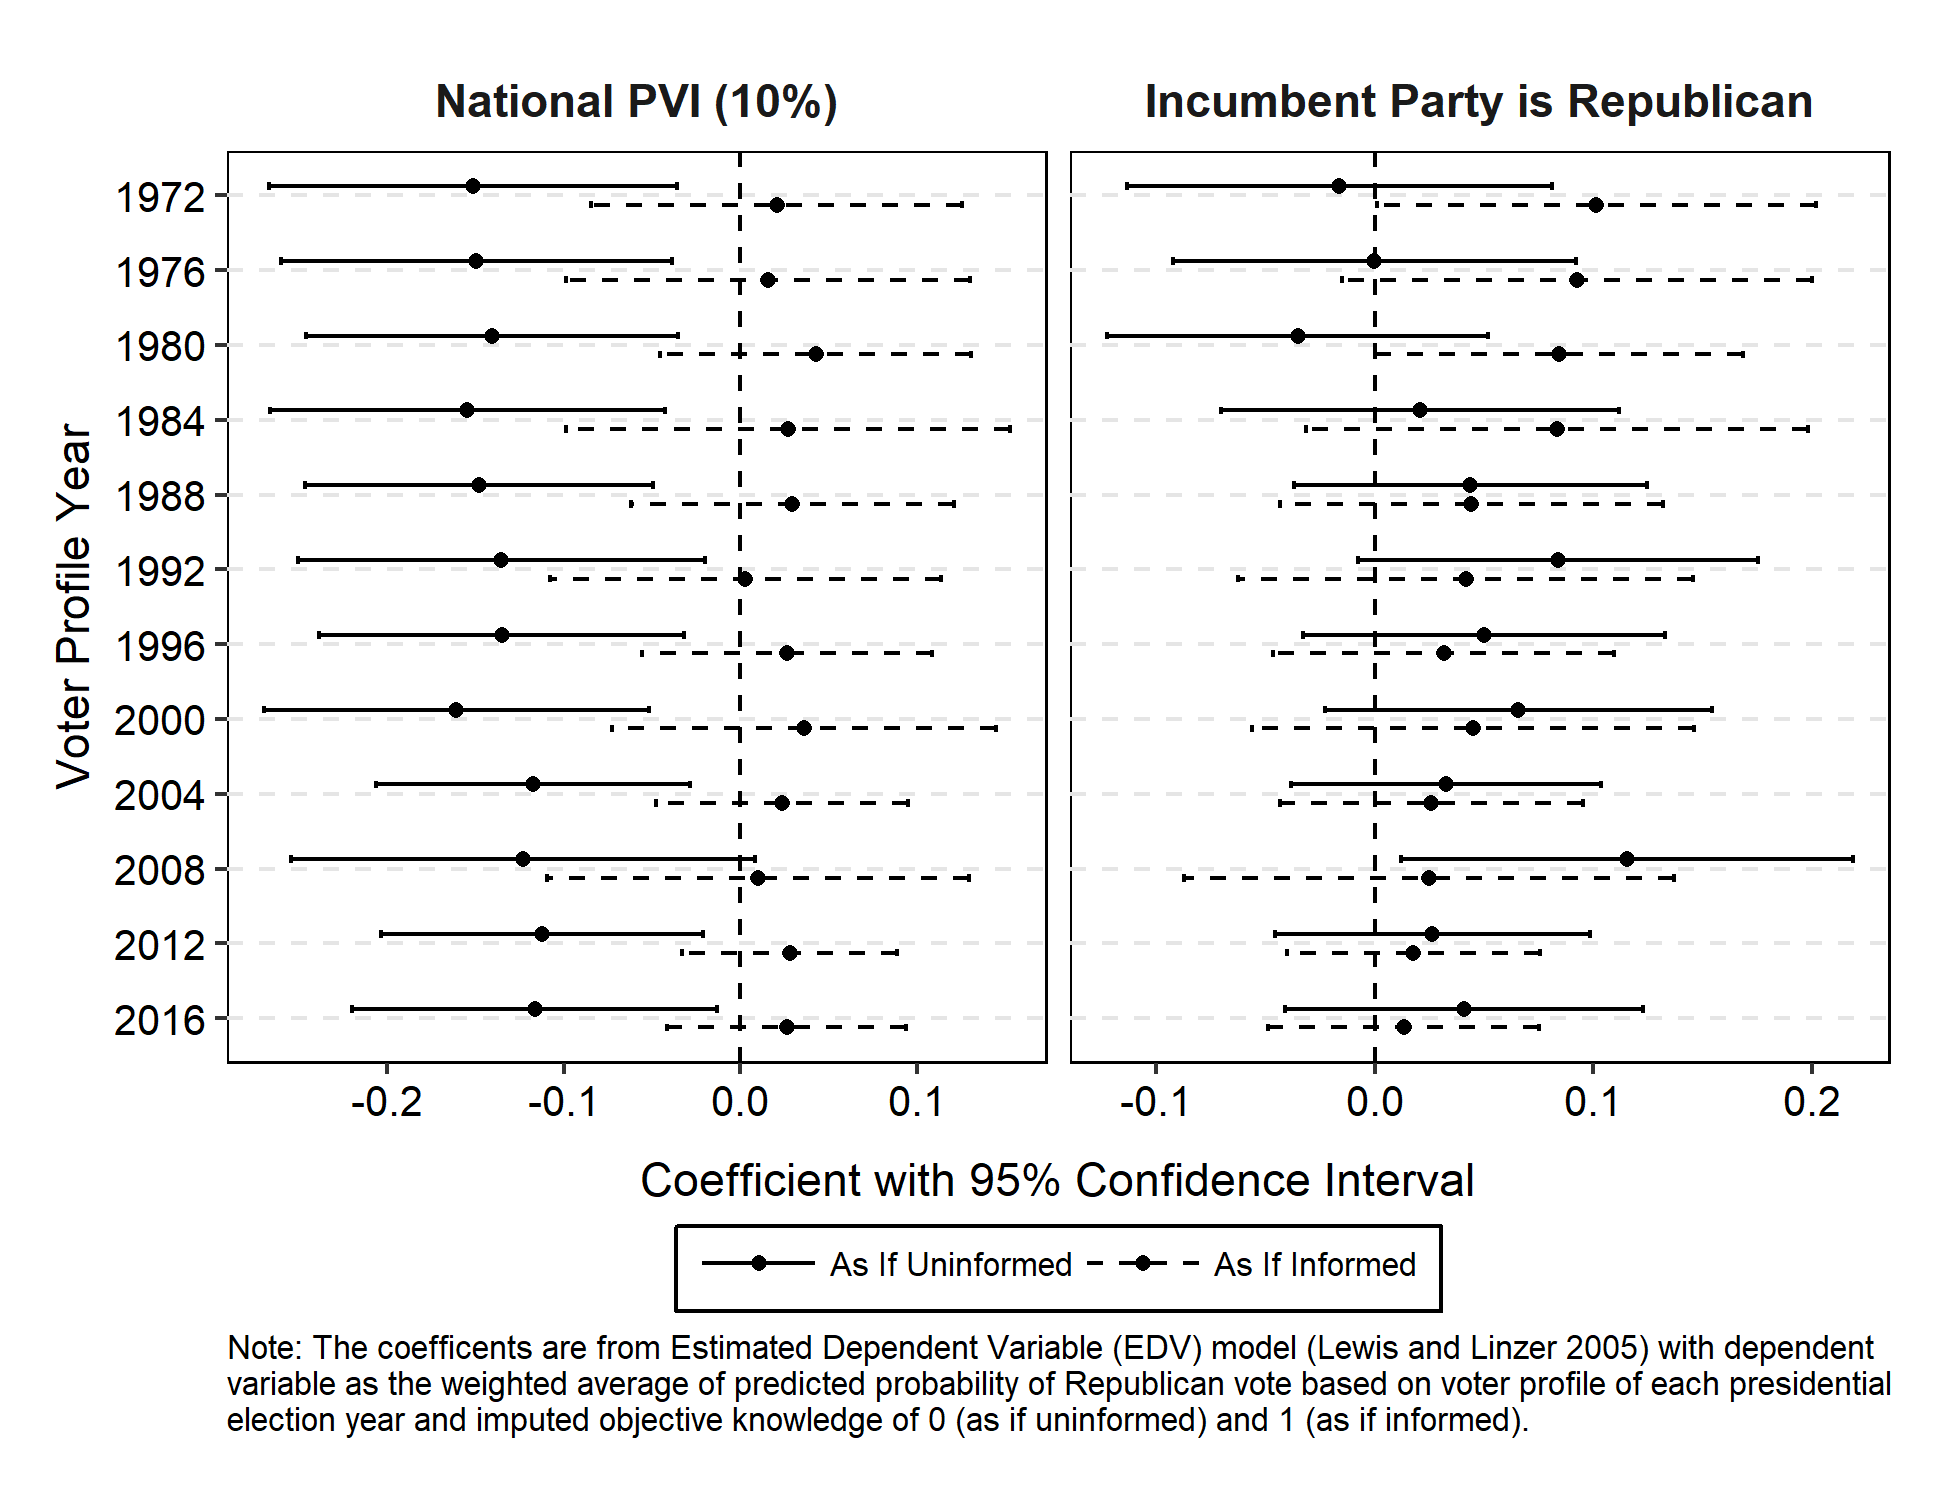
\includegraphics[width=\linewidth]{../outputs/m2sq_anespredtable.png}
\end{figure}



    
\end{document}
